\documentclass[a4paper, 12pt]{article}

\usepackage{amsmath}
\usepackage{graphicx}
\usepackage{geometry}
\usepackage{color}
\usepackage{hyperref}
\usepackage{listings}
\usepackage[none]{hyphenat}
\usepackage[english]{babel}
\usepackage[backend=bibtex, bibencoding=ascii]{biblatex}
\usepackage{csquotes}
\usepackage{lipsum}
\usepackage{chngcntr}
\usepackage{titlesec}
\renewcommand{\familydefault}{\sfdefault}
\newcommand{\sectionbreak}{\clearpage}
\geometry{
	left=1in,
	right=1in,
	top=1in,
	bottom=1in
}

\lstset{
	breaklines=true,
	rulecolor=\color{black}, 
	numbers=left,
	frame = single,
	captionpos=b,
	label=DescriptiveLabel
	}

\lstdefinelanguage{HLSL}
{
	sensitive=true,
	morekeywords=[1]{
	float, float2, float3, float4, float4x4,
	uint, uint2, uint3, uint4,
	RWTexture2D, register, return, if, else
	},
	morecomment=[l]{//},
	morecomment=[s]{/*}{*/},
	morecomment=[l][keywordstyle4]{\#},
}

\counterwithin{figure}{section}

\title{\textbf{Exploration of New Approaches to Depth-Based Render Techniques Utilizing Pixel Synchronization}}

\date{\today}
\author{\textbf{Bryan Pawlowski, Michael Bailey} \\ Computer Graphics \\ \textit{Oregon State University}}

\begin{document}

\begin{titlepage}
\maketitle
\begin{figure}[h]
	\centering
	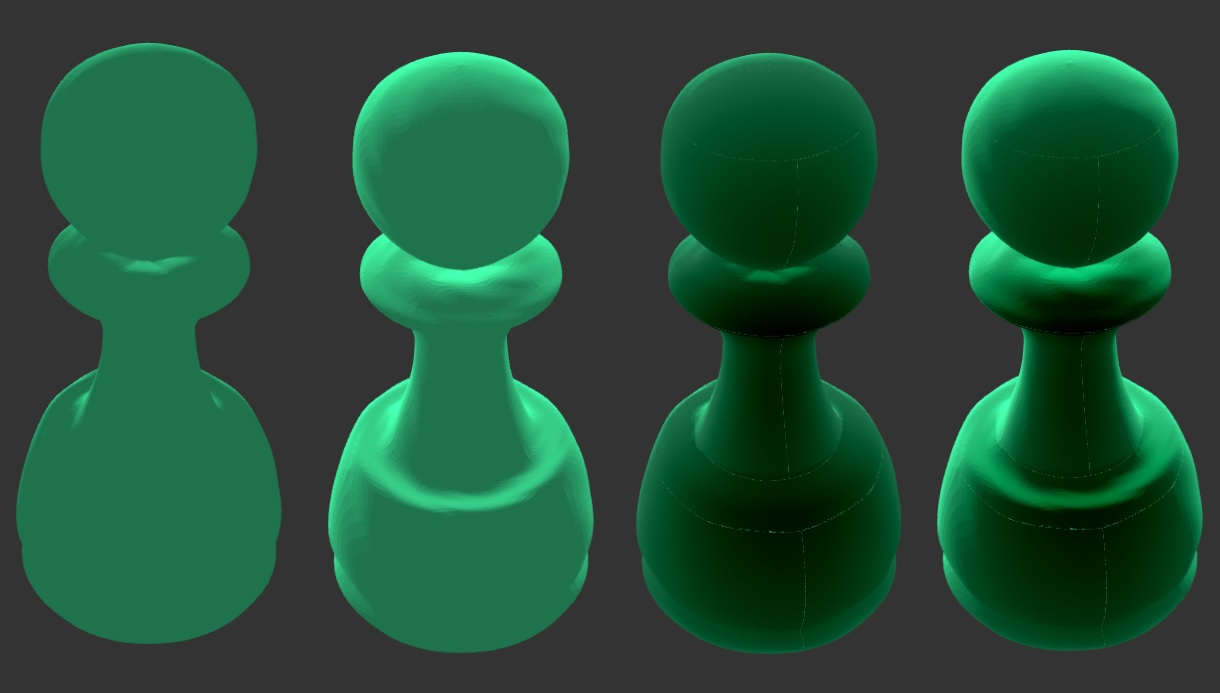
\includegraphics[width=1.0\textwidth]{CloseResult.jpg}
\end{figure}
\thispagestyle{empty}
\end{titlepage}

\pagenumbering{gobble}
\tableofcontents
\pagebreak

\pagenumbering{arabic}

\section{Introduction and Background} 

Since the advent of computer graphics, engineers have been trying to find new
ways to create graphics hardware solutions intended to yield higher
performance and image quality. However, image quality can mean many things to
many people. Individuals may use grapchics hardware to create vibrant and
abstract experiences, where others may create an experience where the images
being created are as photorealistic as possible. The question that graphics
hardware engineers must ask, is, "What can we make that will help developers
create a higher quality experience?" For some GPU distributors, the solution
comes with a concept called Pixel Synchronization. \\ \\ Before we get into
the gory details of what my project is all about, there are some key concepts
that must be covered. This project utilized a lot of different concepts within
Computer Science outside of the realm of graphics. We first need to cover what
the hardware is and why it is different, then take a general look at the
graphics pipeline, and finally discuss two key topics in parallel programming.
My goal is to make sure my rationale for this project is completely clear.

\subsection{Project Environment Details}
\label{hardware}

At the beginning of this project, we did not have any choices, as far as what
chip/chipset on which to run and test our code. The hardware we used has the
Intel\textsuperscript{\textregistered} Core i7, since this CPU/GPU includes
the Iris\textsuperscript{\texttrademark} Graphics Pro 5200. This project was
developed as a desktop application on Windows 8.1, using the DirectX 11 SDK.
Any and all references to Pixel Synchronization calls are done according to
how they are implemented in the Intel DirectX extensions. Within the
application, all HLSL code was compiled using the HLSL version 5.0, as any
lower version does not support the extensions needed to access Pixel
Synchronization.


\subsection{The Graphics Pipeline}

In modern computer graphics, we describe our objects mathematically as a group
of vertices, then pass them to the graphics card where the vertices are
connected and then drawn to the screen, given constraints we have originally
passed. In the beginning, all we, as graphics programmers could do was tell
the GPU to draw, but then our influence on the graphics was over. Later on,
though, the ability to program stages of the pipeline became possible. With
this programmability of the pipeline, graphics programmers now have the
ability to create and define custom effects for the graphics card to carry out
and process.

\subsubsection{The Vertex Shader}

The Vertex shader is the area of entry for every 3D point. Within the vertex
shader, the GPU generally stores the key information and properties of each
vertex, prior to passing it through to the later stages of the pipeline for
these values to be interpolated. The purpose of this, is that it greatly
reduces the amount of space needed to express the looks and properties of an
object. If we can describe the key pieces of information at a few points on
the object, the idea is that the GPU will be able to make informed assumptions
about the other parts of the model where we have provided no information, thus
filling in/connecting the dots.

\subsubsection{The Pixel/Fragment Shader}

Depending on Direct3D or OpenGL, this stage of the pipeline is either called
the Pixel Shader or the Fragment Shader, respectively. Prior to the Pixel
Shader stage, the 3D object has been transformed, and the object's properties
have been interpolated across its entire surface. After this interpolation
takes place, the GPU then decides where, in screen space, the object is, then
runs the pixel shader to color those specific pixels. Most rendering
techniques do most of their lighting effects and color computations at this
stage of the pipeline to help create a smoother coloring of the model. In a
traditional pipeline, the pixels are evluated in parallel, making rendering a
potentially fast process. The tradeoff, however, is that with increased
rendering speed comes a lack of knowledge of other parts of the object being
evaluated. The more naive the pixel is about its neighbors or its
surroundings, the quicker the computation will finish, and the final image
displayed.

\subsection{Parallel Programming}

Pixel Synchronization and my implementation of these different render
techniques borrow concepts from parallel computing. As vertices are passed
through the pipeline and on to the pixel shader, these parts of the pipeline
are actually happening in parallel for all of the different instances of
vertices and pixels. The problem with doing anything depth-based in realtime
graphics, is that each fragment or potential pixel doesn't really have any
knowledge of any of the neighboring pixels, they do not execute in any
specific order, either. In order to know if one potential pixel is deeper than
another potential pixel, we need a predictable way of determining this. If we
were to naively try to gather this information within the pixel shader, we
would run in to a race condition. We also need a way to share this information
across different instances of the pixel shader.

\subsubsection{Shared Resources}

To determine the depth of a certain spot of a 3D model within the pipeline, we
need some sort of a way for the related potential pixels to communicate with
each other. To do this, we use a feature of Direct3D 11 called Unordered
Access Views. Unordered Access Views (UAVs) are basically a read/write texture
that can only be accessed within the GPU, during the Pixel Shader stage. UAVs
can be used in either a 1 or 2 dimensional array. The size of the UAV is
specified to the graphics device before rendering begins. Within the shader,
the programmer must take care to list the UAVs in the same order as they are
initialized within the CPU side of the application. Once properly initialized,
the UAVs are identified within the shader as RWTexture2D data structures.

\subsubsection{Synchronization and Barriers}

Oftentimes, in parallel programs, we must make sure our threads (or in the
case of this project, pixels) are synchronized and executed in some sort of
order. If we know that our programs are executed in some predictable order, it
is easier for us to write more advanced algorithms or have guaranteed
knowledge of what data lies at each checkpoint. If barriers did not exist, we
come across \textbf{race conditions}. When an algorithm is written where race
conditions exist, it is difficult, or impossible to predict the output of the
algorithm, itself.

\subsection{Pixel Synchronization}

\subsubsection{What is Pixel Synchronization?}

With Pixel Synchronization, the pipeline is now capable of creating a barrier
during the pixel shader stage per pixel, where multiple instances of the pixel
being rendered will happen in-order, based on the primitive number. Parallel
programming concepts such as barriers and synchronization have not before been
possible within the real-time pipeline. To have this emerging hardware
capability gives programmers the opportunity to approach existing render
techniques from a new angle, potentially yielding higher performance and more
spectacular images.

\subsubsection{How Pixel Synchronization Works in Code}

\label{section:PixSyncIntro}

\nohyphens{On the programmer side, there is not much coding overhead as far as
initializing, then calling Pixel Synchronization. On the application side, the
programmer must first check the hardware to make sure that the hardware is
capable of Pixel Synchronization. This is the only thing to be done on the
application side. Within the pixel shader, we have to first enable Pixel
Synchronization with a call to \textbf{IntelExt\_Init()}. Then, once we reach
the part of our code that must be syncrhonized, we must call the pixel
ordering function by calling \textbf{IntelExt\_BeginPixelShaderOrdering()}
(\textbf{NOTE:} These function calls are hardware specific. Please see section
\ref{hardware} on page \pageref{hardware} for details about the hardware used
for this project). An important point to keep in mind is that this specific
implementation of Pixel Synchronization lasts until the end of the Pixel
Shader code. What this means, is that it is recommended that all code over
which syncronization must occur should come as close to the end as possible.
Listing \ref{code:PSExample} (below) shows how a bare bones Pixel Shader using
Pixel Synchronization might look. For more information on how Pixel Synchronization works, please rever to section \ref{section:PSBehavior}.}


\begin{figure}[h]
\begin{lstlisting}[language=HLSL]
float4 PSExample(/*parameters...*/) : SV_TARGET
{

	//Variable Definitions

	IntelExt_Init();
	
	//all non synchronization-specific code;

	IntelExt_BeginPixelShaderOrdering();

	//all synchronization-specific code goes here
	//critical section must happen at the end.

	return finalColor;
}

\end{lstlisting}
\caption{How Pixel Synchronization Pixel Shader Code Might Look}
\label{code:PSExample}
\end{figure}

\pagebreak


\section{Simple Subsurface Scattering}

\subsection{What is Subsurface Scattering?}

Subsurface Scattering is a phenomenon which occurs when photons hit some sort
of translucent material, such as skin, fat, milk, plant leaves, etc. The
photons enter that material, scatter, then exit out of a different point. This
phenomenon is constantly and naturally occuring in the real world, but it is a
rather tough lighting effect or phenomenon to calculate in realtime graphics,
since knowledge of the object, and sometimes its surrounding environment, is
required to produce an image with accurate subsurface scattering effects. Even
so, many approximate implementations have been developed to mimic this natural
phenomenon as convincingly as possible, all while retaining
performance/framerate. \\ \\ All of the techniques out there attempt to find a
fast way to build knowledge of the 3D object (what is its depth at a certain
point, and where is it with respect to the light). The techniques that exist
are either quite general, or are very complex, coding wise (further detail to
come below). Pixel Synchronization offers a new approach to the subsurface
scattering problem that is both straightforward and does not sacrifice
performance.

\subsection{Previous Implementations}

As stated above, there exist approaches to approximating the subsurface
scattering effect in realtime graphics. The two approaches detailed below have
trade-offs, when it comes to generality or coding complexity. However, both
methods are quite effective within the correct scope. With the Pixel
Synchronization approach detailed in section 
\ref{section:PSDepthMap} (pg.\pageref{section:PSDepthMap}), we hope to improve
upon these two methods by creating a more detailed and accurate approach,
while keeping the code intuitive.

\subsubsection{Wrapping Approximation}
\label{section:wrapping}
This simple approach to a subsurface scattering approximation takes the
calculation of the diffuse component of your standard Phong lighting equation,
and basically "wraps" the diffuse around the object further than the standart
diffuse calculation. For instance, is illustrated in the equation in Figure
\ref{equation:diffuse} (where $L$ is the light vector and $N$ is the normal
vector).

\begin{figure}[h]
\[diffuse = max(0, L \bullet N)\]
\caption{Standard diffuse calculation in smooth shading}
\label{equation:diffuse}
\end{figure}

\noindent However, when we apply the wrapping approximation, the equation for
the diffuse component is slightly changed. In Figure \ref{equation:wrap}, the
programmer specifies a wrap value, or makes the value interactive to show the
difference in realtime, then the value is applied to the existing equation as
follows:

\begin{figure}[h]
\[diffuse = max(0,((L\bullet N) + wrap) \div (1 + wrap))\]
\caption{Diffuse Calculation in smooth shading with wrap value added}
\label{equation:wrap}
\end{figure}


\noindent As can be seen by observing the above equations, the addition of the
wrapping value in equation complicates it only slightly, but the effect of
adding the is very apparent. The advantage to this approach is that it
requires only a slight modification of Phong illumination. Within shader code,
a graphics programmer could insert a hook in their shader code to show the
difference between Phong Illumination with and without diffuse wrapping. For
an idea on how this is implemented, refer to the code listing in figure
\ref{code:WrapExample}.

\begin{figure}[h]
\begin{lstlisting}[breaklines, language=HLSL]
float calc = dot(Normal, Light) + wrap) / 1 + wrap);
if(mode & DIFFUSE_WRAP) d = max(calc, 0);
else d = max(dot(Normal, Light), 0);
\end{lstlisting}

\caption{HLSL hook to determine whether or not to wrap the normal}
\label{code:WrapExample}
\end{figure}

\noindent In line 2, a bitwise 'and' operator is used to check if wrapping has
been selected because all display mode settings are passed into the graphics
program as a single unsigned integer (in OpenGL, this would be the same as
passing in a single uniform variable to evaluate all user true-false settings.
This saves time and space when passing these types of variables to the GPU). A
more detailed discussion about this and why this approach for uniform
variables is used can be found in section \ref{subsection:Suggestions} on
page \pageref{subsection:Suggestions}, under the "Constant Buffers" item.

\subsubsection{Depth Mapping} 
\label{section:DepthMap}

Given the nature of what Subsurface Scattering is, it is imperative to know
the thickness of the object in question, such that the programmer can make a
decision on how much light escapes the obejct at a different point. For this
reason, a technique was developed called depth mapping. In the first pass, the
scene is rendered from the light's position, toward the object, where we store
the distance from the light to that location on the object. Another pass is
made to measure where the ray has entered and exited, by mapping the depths to
the object's texture space. Finally, in the render pass, we render the object
from the camera's point of view, and for each point on the object being
rendered, we find the point of entry and the point of exit for the specific
ray pertaining to the current fragment of the object, then calculated the
distance between the two. After this distance has been calculated, the new
calculation of the diffuse light can be applied. For a visual representation
of the render pass of the approach, see figure \ref{pic:DepthMap} on page
\pageref{pic:DepthMap}. \\ \\ The effect from this approach causes more of a
subsurface scattering type of "lifelike glow" than the method detailed in
Section \ref{section:wrapping}. However, when this method is implemented, it
requires three passes to render the image with correct depth information.
Further, there is no intuitive way to project the the depth information with
respect to the light to the object. To recap, here are the three render passes
that take place.



\begin{figure}[h]

\begin{description}

\item[First Pass] \hfill \\ Render the object from the perspective of the
light and record the distances from the light.

\item[Second Pass] \hfill \\ Calculate the distances between the entry and
exit points of the light rays. These will be mapped, in texture space, to the
object.

\item[Third Pass] \hfill \\ Use the depth calculations to scale the backfacing
(with respect to the light) diffuse component of the object.

\end{description}
\caption{Description of the depth mapping approach to subsurface scattering}
\label{figure:depthDesc}
\end{figure}

\begin{figure}[h!]
	\centering
	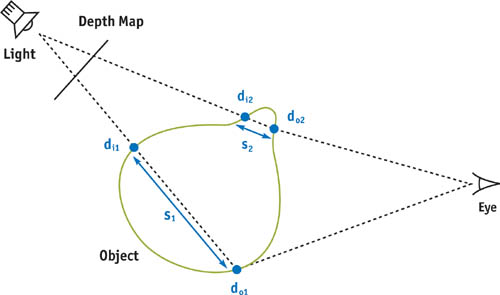
\includegraphics[width=1.0\textwidth]{depthMap.jpg}
	\caption{Diagram to visualize how the depth map is used to calculate the distance a light ray has traveled within a 3D object}
	\label{pic:DepthMap}
\end{figure}



\subsection{Pixel Synchronization Accelerated Depth Mapping}
\label{section:PSDepthMap}

The approach described in section \ref{section:DepthMap} is the groundwork for
the new Pixel Synchronization accelerated approach. The concept remains
relatively the same, however, we are able to use a psuedo raytrace to guage
the distance between two points in the same ray with increased ease. This more
straighforward approach to depth mapping takes less time to code and yields no
loss of performance.

\subsubsection{In-Depth Description of Implementation}

As stated above, the approach to this technique remains generally the same,
but with a few differences. For clarity's sake, refer to the description in
\ref{figure:depthDesc} as a reference to what the changes in the pixel shader
based approach would be, in comparison to the description below.

\begin{figure}[h!]

\begin{description} 

\item[First Pass] \hfill \\ 

This pass remains relatively the same. We take this pass to map which pixel
from the perspective of the light. However, we map the object to the screen
with respect to its texture coordinates. This way, we guarantee that all of
the object is being seen and processed by the GPU. For a better idea of what
this means, see the listing \ref{code:VShaderPSDepth} on page
\pageref{code:VShaderPSDepth}. More specifically, see lines 6 through 8. Here,
we take the text coordinates, then convert them into a space spanning from -1
to 1 in the x and y axes. Then, when these positions are passed from the
vertex to the pixel shader, they are converted to screen space. \\ \\ After
this screen space conversion, we calculate and store the distance of each part
of the model from the light source. Following this, we then map which rays
intersect which parts of the model in 3D space. This is why we also store and
keep track of the 3D position of the model, as seen on line 11 in listing
\ref{code:VShaderPSDepth}. We map these ray values (which coincide with the
pixels) to another texture, which we will use in the next pass as a "mask."
For an idea of these mappings, refer to \ref{code:PixelShaderPSDepth} on page
\pageref{code:PixelShaderPSDepth}. We use Unordered Access Views to accomplish
these mappings (\ref{section:UAVs}, page \pageref{section:UAVs}).

\item[Second Pass] \hfill \\  

This pass is from the perspective of the light, but this time, we project the
correct object into space, rather than its texture coordinates. The only
difference here, is that $output.svposition$ gets $mul(final, position)$
rather than the calculated screen space coordinates as it does in line 9 of
figure \ref{code:VShaderPSDepth}. However, within the Pixel Shader this time,
we create our shallow mask. This is basically a UAV-created depth buffer to
keep the shallowest positions with respect to the light. To see how this is
implemented within the shader, please see listing \ref{code:POShader} on page
\pageref{code:POShader}. With the aid of Pixel Synchronization, we can determine which parts of the object are closest to (facing) the light.

\item[Third Pass] \hfill \\ 

The final render pass remains the same as what we had in the approach on page
\pageref{section:DepthMap}. We take the current depth, with respect to the
light, then compare it to the corresponding member of the shallow mask. For a
coding example, turn to page \pageref{code:PSDepthRender} and see figure
\ref{code:PSDepthRender}. The code block from lines 6 to 25 show how to both
get the ray and the current light-based depth of the object, compare them, and
then re evaluate the diffuse component, originally calculated above this
section Other parts of the shader were edited out for the sake of readability
and clarity. There will be a complete discussion on the code within
$PSHader2()$ later on in this paper. We can get away with using array
notation, since UAVs support access via array notation, and not with a call to
$sample()$.

\end{description}
%\caption{Description of the depth mapping approach to subsurface scattering}
\label{figure:PSDesc}
\end{figure}

\begin{figure}[h]
\begin{lstlisting}[breaklines=true,language=HLSL]
float4 PShader2(...)
{

	/*...*/

	if (!(mode & PHONG_RENDER))
	{
	  uint2 lightCoords;

	  lightCoords.x = fromLightX[uv];
	  lightCoords.y = fromLightY[uv];

	  float mdepth = uvDepth[uv];

	  float shallow = Shallow[lightCoords];
	  if ((mode & PIXSYNC_OFF) && 
	      (uvDepth[uv] > Shallow[lightCoords])){
		  
		  float4 lColor = lightcol;
		  lColor -= 
		    (uvDepth[uv] - Shallow[lightCoords]) * 3;
			
		  diffuse += lColor;
	  }
	}

	/*...*/
}
\end{lstlisting}

\caption{Render Pass from perspective of camera}
\label{code:PSDepthRender}
\end{figure}

\pagebreak

\section{Refraction}

Refraction is a visual phenomenon that occurs when a translucent object, such
as a glass figurine, bends light in such a way that it distorts the image
beyond it. This is how real-life lenses accomplish vision correction, or the
image of an object gets distorted when it is submerged in water. As humans, we
rely on refraction a great deal, so we are very, very used to seeing this
effect on a day-to-day basis. There are many ways to accomplish the
approximate effect of refraction on the GPU. The first approach, detailed in
section \ref{section:SimpleRefract}, is a simple refraction algorithm, that
takes into account only the front face of the object to compute the color of
the object at that point.

\subsection{"Fake" Convex Object Refraction}
\label{section:SimpleRefract}

The most used approach to refraction is to just bounce the viewing "ray" once
on the front surface of the object, then samples the cubemap to return a
color. In code, this effect requires just a Vertex and Pixel Shader.

\subsubsection{Vertex Shader}

All of the heavy-lifting for refraction is done within the Vertex Shader
(\ref{code:VSSimpleRefract}). Given the proper transform and rotation
matrices, the refract vector is computed within the Vertex shader.
Essentially, the distance between

\begin{figure}[h]
\begin{lstlisting}[breaklines=true,language=HLSL]
VOUT VShader(...)
{

	VOUT output;

	output.svPos = mul(WVP, pos);
	output.Pos = mul(WVP, pos);
	float4 norm = mul(Rotation, normal);


	float diffusebrightness = 
			saturate(dot(norm, LightVector));

	float3 ECPosition = mul(World, pos).xyz;
	float3 eyeDir = float3(0.0f, 0.0f, 0.0f) - ECPosition;
	
	output.Color = AmbientColor;

	output.Color += LightColor * diffusebrightness;
	output.Normal = norm;
	output.texCoord = texCoord;

	float3 reflectVector = refract(norm, eyeDir, -.90);

		output.vRef = reflectVector;


	return output;
}
\end{lstlisting}

\caption{Vertex shader for simple refraction}
\label{code:VSSimpleRefract}
\end{figure}

\begin{figure}[h]
\begin{lstlisting}[breaklines=true,language=HLSL]
float4 PShader( VOUT input ) : SV_TARGET
{	
	float3 bounceVec = input.vRef.xyz;
	
	float4 newColor = 
	 SkyMap.Sample(ObjSamplerState, normalize(bounceVec));
	
	return newColor;
}
\end{lstlisting}

\caption{Pixel shader for simple refraction}
\label{code:PSSimpleRefract}
\end{figure}

\subsection{Better Convex Refraction With Pixel Synchronization}

The idea behind this approach is to create a volumetric representation of the
scene which stores the object's surface normals, with respect to the eye. For
the render step, we could step through this voxelization at the entrypoint,
then trace the first refracted ray to the exit point, refract again, then
return this double-refracted color to give a more accurate coloring of the
pixel.

\subsubsection{Shader-Based Description of Implementation}

To get our volumetric representation, I attempted (see section
\ref{subsection:Implementation} for more details) to utilize the shader to
take care of that for me. Using Pixel Ordering, I tried to create a voxel-
based representation of the entire scene. I tried to use two 3D textures to
accomplish this. One 3D texture would have $unsigned int$ representations of
every voxel element saying whether it was inside, outside, or on the face of
the object within the scene:

\begin{description}
\item[0:] outside of the object
\item[1:] on the object's face
\item[2:] inside of the object
\end{description}

\noindent The suface normals are stored in another 3-D texture. We would first
mark all of the spaces according to the above description. The surface normal
texture is populated at the beginning of populating this unsigned integer
texture. How this texture is populated can be better described by the code
within figure \ref{code:3DTexPop}. On line 8, we begin our loop to populate
the 3D texture. As can be seen, pixel ordering has been invoked within this
shader. So, what we do is step through our $unsigned int$ Texture3D at every
pixel address, in order. this way, we are able to indicate which parts of the
scene are inside or outside of the model. We keep another 3D texture to keep
track of the surface normals. The idea behind this, was once we hit an index
in the $unsigned int$ Texture3D of value 1, we could then use that index where
the 1 value is to refract the ray further, since that is where the surface
normal at that point is stored in the other Texture3D. Using these textures in
tandem serves as a good way to trace through a solid object to find the
accurate refraction. However, I didn't get as far as a tracing stage to my
algorithm, as there are fundamental aspects of this algorithm that GPU
compilers do not allow to happen, due to memory access restrictions. This will
be covered in more detail in section \ref{subsection:Implementation}, where
the implementations will be discussed. However, the source code for this
attempted demo will still be included in my final source code.

\begin{figure}[h]
\begin{lstlisting}[breaklines=true,language=HLSL]
float4 PShader(...)
{

	IntelExt_Init();
	IntelExt_BeginPixelShaderOrdering();

	/*...*/

	uint3 tempi = voxPos;

	[loop]
	for (i = voxPos.z + 1; i < 512; i++)
	{
		tempi.z = i;
		unsigned int cond = VoxMask[tempi];
		if (cond == 0)
		{
			VoxMask[tempi] = 2;
			continue;
		}
		else if(cond == 2)
		{
			VoxMask[tempi] = 0;
			continute;
		}
		break;
	}
	/*...*/
}
\end{lstlisting}
\caption{Populating the \textit{unsigned int} 3D texture.}
\label{code:3DTexPop}
\end{figure}

\section{Implementation Discussion}
\label{section:ImplementationDiscussion}

This section will detail important parts of code in-depth such that a majority
of questions may be answered. The idea is that another student may be able to
pick up the code I have implemented and quickly understand what decisions were
made and why, which pieces of code depend on others, and so on. This way,
changes can be made in an effective, informed manner, rather than with a
trial-and-error approach, which can prove to be far less efficient.

\subsection{Boilerplate Code}
\label{subsection:BoilerPlateImplementation}

A majority of the Boilerplate functionality stays consistend between the two
code bodies. As this is the case, the explanation of code setup,
initialization and variable meanings will take place here. However, this
section must not be considered to be a comprehensive tutorial on DirectX, but
help explain some of its differences to OpenGL, as the latter is used in this
University's Curriculum.

\subsubsection{Defining our Window}

This code is straightforward, but could seem a bit foreign to a programmer who
has not programmed in windows before. Right at the beginning of the program,
two things must happen. Firstly, a window class must be defined and then
registered with the operating system as seen in figure  \ref{code:winClass}.
Within this code snippet, the important lines are 6, 7, and 12.

\begin{description}

\item[Line 6:] Here, the programmer is stating that this window will be 
redrawn.

\item[Line 7:] This is a pointer to a separate function called WindowProc.
WindowProc is where all of the messages and interactions with that window
will be coded. In other words, WindowProc will execute every time there is a
message to the window.

\item[Line 12:] This is where the program attempts to register the window
class with the operating system. In otherwords, this determines whether the
program has permission to create windows of this type of class.

\end{description}

\noindent If successfull with this portion, the program may now attempt to
create a window instance, as seen in the code snippet in figure
\ref{code:CreateWindow}. After the variable, $hWnd$, has been populated, it
will be used later to link a D3D device. Another point worth noting is that
the window size used was 1920x1080, as part of this project was to ensure that
this effect could be used on a window size that is commonly used within
industry for video games and scientific visualizations.

\begin{figure}[h!]
\begin{lstlisting}[language=C++]
WNDCLASSEX wc;

ZeroMemory(&wc, sizeof(WNDCLASSEX));

wc.cbSize = sizeof(WNDCLASSEX);
wc.style = CS_HREDRAW | CS_VREDRAW;
wc.lpfnWndProc = WindowProc;
wc.hInstance = hInstance;
wc.hCursor = LoadCursor(NULL, IDC_ARROW);
wc.lpszClassName = L"WindowClass";

if (!RegisterClassEx(&wc))
{
	int nResult = GetLastError();
	MessageBox(NULL,
		L"DirectX window class creation failed\r\n",
		L"Window Class Failed",
		MB_ICONERROR);
	exit(EXIT_FAILURE);
}
\end{lstlisting}

\caption{Creating and registering a Window Class}
\label{code:winClass}
\end{figure}

\begin{figure}[h!]
\begin{lstlisting}[language=HLSL]
RECT wr = { 0, 0, SCREEN_WIDTH, SCREEN_HEIGHT };
AdjustWindowRect(&wr, WS_OVERLAPPEDWINDOW, FALSE);

hWnd = CreateWindowEx(NULL,
	L"WindowClass",
	L"Pawlowski Pixel Ordering Research",
	WS_OVERLAPPEDWINDOW,
	300,
	300,
	wr.right - wr.left,
	wr.bottom - wr.top,
	NULL,
	NULL,
	hInstance,
	NULL);

ShowWindow(hWnd, nCmdShow);
\end{lstlisting}
\caption{Create and Show the Window}
\label{code:CreateWindow}
\end{figure}

\subsubsection{Direct3D Setup}

When the program is ready to initialize direct3D, all it needs is for the
calling process to pass the pointer to the window instance to which the
Direct3D device will be tied. As there is a very excellent
\href{http://www.directxtutorial.com}{tutorial website}(listed below), There
will not be any code included within this portion. \\ \\ The most important
difference between Direct3D and OpenGL is the use of COM Objects. COM
(Component Object Model) Objects are Microsoft's way of making interprocess
communication, or even IO with peripherals easier. In this case, Direct3D
devices are represented with COM objects. As this is the case, there are
slightly different ways to interact with the GPU when using Direct3D. For more
information, please refer to
\href{http://www.directxtutorial.com}{http://www.directxtutorial.com}, or
microsoft's \href{https://msdn.microsoft.com/en-
us/library/windows/desktop/ms690343(v=vs.85).aspx}{own documentation} online.

\subsubsection{Constant Buffer Values Explained}

For this code base, the same Constant buffer was used for each of the
demonstrations bundled within the SSS visual studio project. This decision was
made because a good number of the values within the constant buffer were re-
used in the other demonstrations. That said, there are many values within this
constant buffer. The constant buffer is defined in both the application and
the shader as follows:

\begin{lstlisting}[language=C++, numbers=none, frame=none]
__declspec(align(16))
struct CBUFFER
{
	D3DXMATRIX Final;
	D3DXMATRIX Rotation;
	D3DXMATRIX modelView;
	D3DXVECTOR4 LightVector;
	D3DXCOLOR LightColor;
	D3DXCOLOR AmbientColor;
	D3DXVECTOR4 LightPos;
	unsigned int mode;
};
\end{lstlisting}

\noindent The first line, \textbf{\_\_declspc(align(16))}, is included to
demonstrate yet another way to avoid the Constant Buffer creation error, where
a struct is not of a size that is divisible by 16, as detailed in the
"Constant Buffers" item in section \ref{section:suggestions}. A majority of
these member values are easy to understand their use; however, there is one
value, \textbf{mode}, whose utility is not as readily apparent. \\ \\ Since
there are conditions as far as what technique to use, or what to render, this
could be a rather space-consuming constant buffer, if each condition were to
be stored inside of its own variable. However, with bitmasking and bitwise
arithmetic, all of these boolean values can be stored in a single integer. For
more information on how the bitmasked values are set up, refer to the
DXApp.cpp file included in the SSS directory of the project. All values are
set to a certain bit, which means that they are all contiguous powers of two.
This approach for storing booleans is a benefit in that it is not time or
space intensive for the Application to send these boolean values to the GPU.

\subsection{SubSurface Scattering Shader Walkthrough} 

\label{subsection:SSSImplementation}

\subsubsection{Pass 1}

For the first render pass, texture-based knowledge of the model must be
stored. As will be detailed in section \ref{subsubsection:BadRender}, this
pass was added to ensure all texture space is covered when passing the model
through the pipeline. Within this pass, the scene is projected from the
perspective of the light, toward the object. After the model has been
transformed, the texture coordinates of each vertex is passed throught he
pipeline as the X and Y of the SV\_POSITION HLSL semantic. This maps the
entire surface of the model to the viewport. If this pass were to be rendered
to the screen, it would look like figure \ref{pic:texSpace}. As can be seen,
the different portions of the pawn model are easily discernable. However,
other objects take the entire screen space, as seen in figure
\ref{pic:cubeTSpace}. 

\begin{figure}[!htb]
	\centering
	
\includegraphics[width=1.0\textwidth]{textureSpace.jpg}
	\caption{Pawn Model's Surface Unwrapped With Respect to Texture Space}
	\label{pic:texSpace}
\end{figure}

\begin{figure}[!htb]
	\centering
	
\includegraphics[width=1.0\textwidth]{cubeTSpace.jpg}
	\caption{Cube Model's Surface Unwrapped With Repsect to Texture Space, Shown to Illustrate a Model Whose Surface Spans the entire texture coordinate range}
	\label{pic:cubeTSpace}
\end{figure}

\noindent Mapping the model's surface to the screen through texture space is a
necessary step, as it guarantees that all of the model is rendered, thus
information is stored at all possible locations in the model's texture space.
The results of the implementation in section \ref{subsubsection:BadRender}
will illustrate why this pass is necessary. \\ \\ In figure
\ref{code:VShaderPSDepth}, the key code lines are lines 5 through 9. Here, the
program is converting the texture coordinates to a value ranging from -1 to 1,
which forces the texture coordinates to be interpolated and displayed on the
screen. On line 10, the program is ensureng that the 3D coordinates are still
being passed through. These coordinates are given an orthogonal projection.
This is key for storing which portions of the model are on which pixel
position if the model were to be projected correctly into screen space through
the pipeline. In other words, the program is keeping track of the model's 3D
position, such that it can be used to store information within the pixel
shader. \\ \\ The Pixel Shader for this pass, figure
\ref{code:PixelShaderPSDepth}, the program finds what the screen-space
position should have been for the correctly projected 3D model (lines 3, 7
through 9, 13 and 14) and stores them into UAV textures representing the X and
Y coordinates of the model's screen position from the perspective of the light
(lines 16 and 17). These values are stored as individuals, as tuples have a
difficult time being used in a UAV when using Pixel Synchronization. These are
stored at the texture coordinates, as texture coordinates stay at the same
location of the model's surface, regardless of the model's orientation in
space. Lastly, the depth with respect to the light's position is stored in a
depth UAV. Writing this pass to the screen yields a result that can look
somewhat like an abstract painting, such as figure \ref{pic:logTSpace}.

\begin{figure}[!htb]
	\centering
	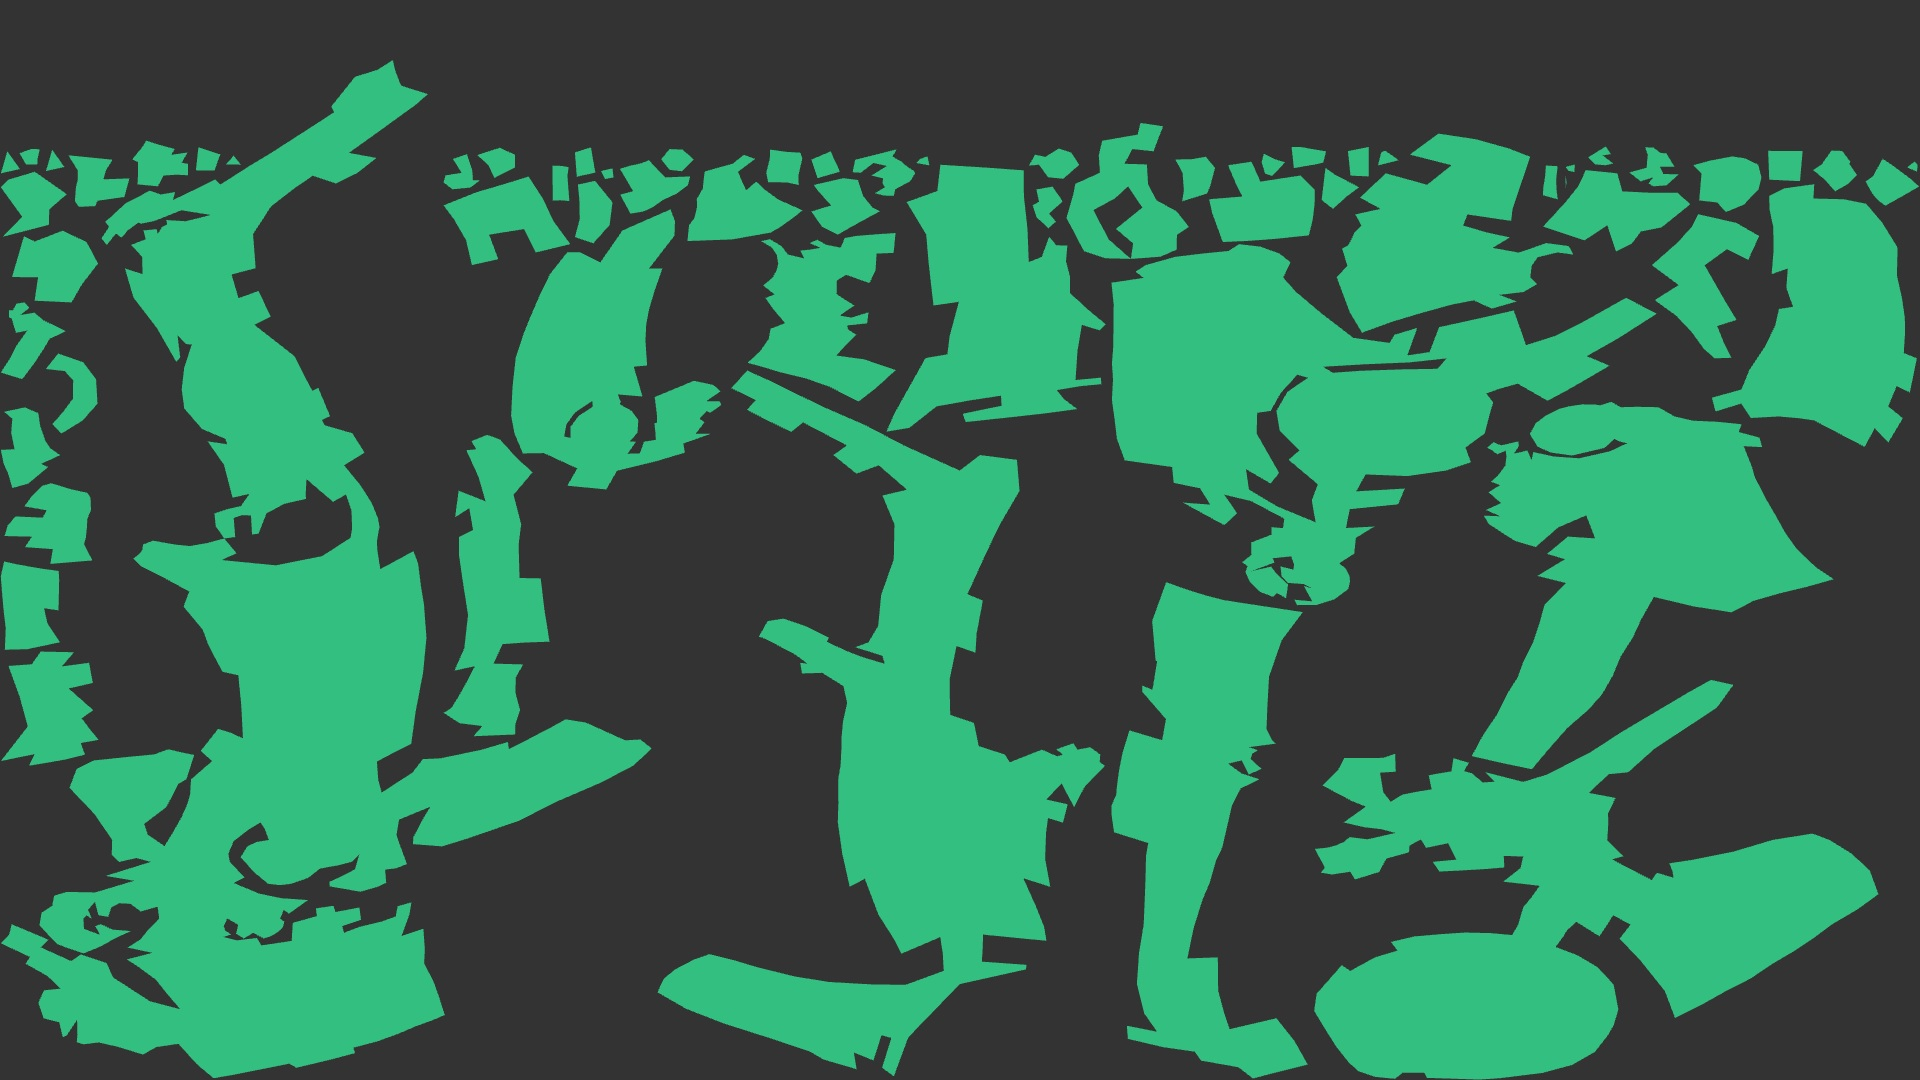
\includegraphics[width=1.0\textwidth]{logTSpace.jpg}
	\caption{Log Model's Surface Unwrapped With Repsect to Texture Space}
	\label{pic:logTSpace}
\end{figure}

\begin{figure}[!htb]
\begin{lstlisting}[breaklines=true, language=HLSL]
VOut VShader(...)
{
	VOut output;

	float2 movedCoords = texCoord * 2;
		movedCoords.x -= 1;
		movedCoords.y -= 1;
	float4 svPos = float4(movedCoords, 0.0, 1.0);
	output.svposition = svPos;
	output.position = mul(final, position);

	// set the ambient light
	output.color = ambientcol;

	
	float4 norm1 = normalize(mul(rotation, normal));
	float diffusebrightness = saturate(dot(norm1,lightvec));
	float4 norm = normalize(mul(final, normal));

	//output.color += lightcol * diffusebrightness;

	output.UVs.x = texCoord.x * SCREEN_WIDTH;
	output.UVs.y = texCoord.y * SCREEN_HEIGHT;

	output.normal = norm;

	output.camera = mul(final, lightPos);

	output.mode = mode;


	return output;
}
\end{lstlisting}
\caption{Vertex Shader for first Pass of Depth Map accelerated by Pixel 
Synchronization}
\label{code:VShaderPSDepth}
\end{figure}

\begin{figure}[!htb]

\begin{lstlisting}[breaklines=true, language=HLSL]
float4 PShader(...) : SV_TARGET 
{
	float2 svPos = position.xy;
	float mdepth = distance(position, camera);
	uint2 uv = UVs;

	svPos.y = 0 - svPos.y;
	svPos += 1;
	svPos = svPos / 2;

	float2 newPos;

	newPos.x = svPos.x * SCREEN_WIDTH;
	newPos.y = svPos.y * SCREEN_HEIGHT;

	fromLightX[uv] = newPos.x;
	fromLightY[uv] = newPos.y;
	uvDepth[uv] = mdepth;

	return color;
}
\end{lstlisting}
\caption{Pixel Shader from first pass of Pixel Synchronization-Accelerated 
depth mapping.}
\label{code:PixelShaderPSDepth}
\end{figure}

\subsubsection{Pass 2}

Now that depth information regarding the model has been gathered, the second
pass is where the pixel synchronization happens. The vertex shader in this
pass stays relatively the same as the previous pass; however, the projected
model coordinates are passed to the SV\_POSITION semantic, rather than the
converted texture coordinates, as in the previous pass. To see how the shallow
buffer is created, refer to figure \ref{code:POShader}. Within this pixel
shader, the depth with respect to the light is recorded for every pixel/
fragment. Then, the pixels are ordered, and then shallowest depth at that
pixel location is recorded.

\begin{figure}[!htb]
\begin{lstlisting}[breaklines=true, language=HLSL]
float4 POShader(...) : SV_TARGET
{
	uint2 pixelAddr = svposition.xy;

	float pos = distance(position, camera);

	IntelExt_Init();
	IntelExt_BeginPixelShaderOrdering();

	if (pos < Shallow[pixelAddr])
	{
		Shallow[pixelAddr] = pos;
	}

	return color;
	
}

\end{lstlisting}
\caption{Pixel Ordering step of the alternate approach to depth mapping}
\label{code:POShader}
\end{figure}

\noindent The main purpose of this pass is to map which part of the model is
shallowest to the light at a certain pixel position. With the utilization of
pixel synchronization, this is a very straightforward process, with a
guarantee against race conditions. With the help of the information gathered
from the previous pass, the indexing and access of this information is
straightforward. The image that would be output to the screen is far less
interesting than the texture-space rendering, as it is an orthogonal view of
the object from the perspective of the light, as seen in figure
\ref{pic:orthoPawn}. The purpose of the orthogonal projection is such that we
get a true trajectory of the light through the model, and not a trajectory
that follows perspective foreshortening. It is important to note that, within
this pass, the object must be contained within the boundaries of the view
volume, otherwise key texture-based information will be missed for large
portions of the model. However, it is important to maximize the amount of
screen space filled by the model for this path, to give as detailed depth
information as possible.

\begin{figure}[!htb]
	\centering
	
\includegraphics[width=1.0\textwidth]{orthoPawn.jpg}
	\caption{Orthogonal Projection of Pawn Model with repsect to the light.}
	\label{pic:orthoPawn}
\end{figure}

\subsubsection{Pass 3}

\label{section:SSSPass3}

For the final pass, the graphics program applies phong illumination from the
perspective of the eye position with a perspective foreshortening projection.
In addition to phong illumination, the depth-based calculations are applied to
the final colors of the image, as well. To keep things simple, the color's
diffuse brightness is scaled based upon its orientation to the light, and its
model-specific depth, based upon that orientation. As this is a modified Phong
Illumination technique with added depth information, the Vertex Shader is
nothing different from what has already been seen. The same Pixel Shader,
PShader2(), is used for three different render modes. Figure
\ref{code:SSSFinal} details the portion of the shader that adds the depth
information to the coloring of the image. As such, each section will discuss a
different piece of the greater pixel shader function.

\begin{figure}[!htb]
\begin{lstlisting}[language=HLSL]

			    /*...*/

if (!(mode & PHONG_RENDER))
{
	uint2 lightCoords;

	lightCoords.x = fromLightX[uv];
	lightCoords.y = fromLightY[uv];

	float mdepth = uvDepth[uv];

	float shallow = Shallow[lightCoords];

	if ((mode & PIXSYNC_OFF) && 
		  (uvDepth[uv] > Shallow[lightCoords])){

		float4 lColor = lightcol;
		lColor -= (uvDepth[uv] - 
			Shallow[lightCoords]) * 3;
			
		diffuse += lColor;
	}
}

			    /*...*/

\end{lstlisting}
\caption{Chunk of Pixel Shader for final pass of the the Pixel Ordering-powered Subsurface Scattering technique}
\label{code:SSSFinal}
\end{figure}

\noindent \\ In this portion of the pixel shader, the program is checking to
see if the SubSurface Scattering effect is activated. If so, the XY
coordinates for the part of the model that is being processed (with respect to
the light's view), the depth, and the shallow buffer are all referenced. The
depth difference is then calculated and exaggerated by a factor of 3. The
constant 3 was chosen in this case, as this best illustrated the effect
without making it too exaggerated or underexaggerated. The variable, $lColor$,
then subtracts this value from all of its components, then this color is added
to the diffuse component of the pixel's final coloring. This is because when
the subsurface scattering phenomenon takes place, the 'glow' of the object
does take influence from the color of the light, as well as the object's
diffuse color.


\subsection{Bad Render Function and Shader Walkthrough}
\label{subsubsection:BadRender}

This first attempt at utilizing pixel shaders was retained within the project
to prove why the initial information gathering pass is so necessary. For the
sake of speed, it seems as though the graphics pipeline, on the hardware on
which this project was run, makes choices to round some values. As this is the
case, there are coordinate values that do not get properly interpolated across
the pipeline. This results in texture holes, as members of the UAV do not end
up being populated. For an idea of what this would look like, refer to figure
\ref{pic:pBadRender}.

\begin{figure}[!htb]
	\centering
	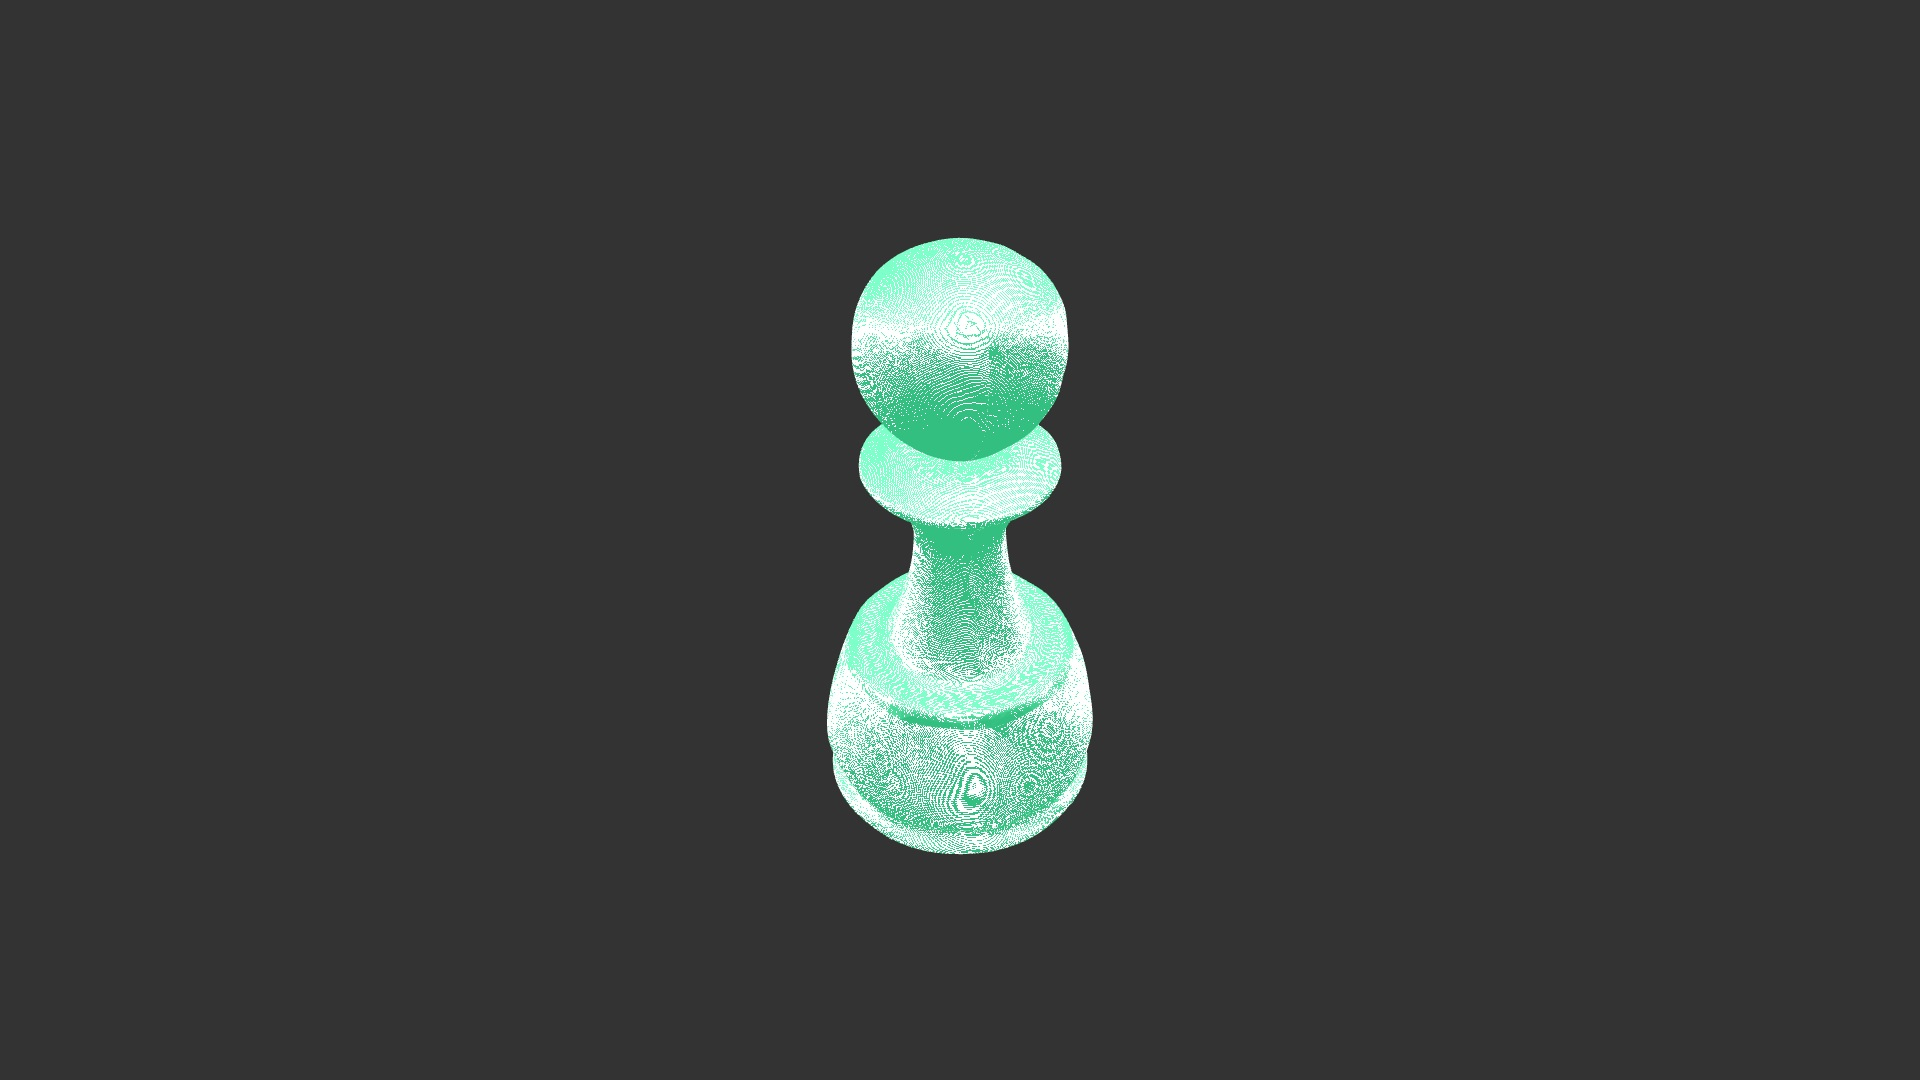
\includegraphics[width=1.0\textwidth]{pBadRender.jpg}
	\caption{Pawn Rendered with the Attempted 2-Pass technique, colors exaggerated to better show the negative effect of this attempt.}
	\label{pic:pBadRender}
\end{figure}

\noindent The hypothesis that the pipeline was causing texture holes was
corroborated when the unwrapping of the model's surface with respect to
texture space was completed. As soon as the model was first unwrapped, then
pixel synchronization based upon depth was taken into account, all texture
holes disappeared, giving a consistent, cohesive shadow/glow effect from the
subsurface scatter approximation. Further attempts were made to make this
implementation work, such as forcing the pipeline optimizations to be turned
off, but not attempts yielded any different results in the image. For a larger
version of figure \ref{pic:pBadRender}, refer to page
\pageref{pic:bigBadRender}. 

\subsection{Culling Demo Render Function and Shader Walkthrough}

This demo was implemented to test to raw effect of pixel synchronization on
the performance of the graphics pipeline. The performance results can be seen
above. This demo had three different modes. One was a "No Cull" mode, which is
self-explanatory. This mode was included in the demo, such that a measurement
of performance could be taken when all of the model is rendered. There is a
"Hardware Cull" mode, where measurements are taken for performance as well.
All performance measurements are taken to compare against the "Software Cull"
mode. The Software Cull mode is where culling within the shader takes place,
witht he help of Pixel Synchronization. The purpose of culling within the
shader was to give a visual result between the "No Cull" and the "Software
Cull" modes. \\ \\ The "Software Cull" mode utilizes 2 UAV textures. One is a
clear mask, and the other keeps track of the shallowest depth. The code in
figure \ref{code:softCull} demonstrates how this works. In short, if the
software cull flag is set, the shader program accesses the ClearMask UAV to
see if another pixel at that location had been previously processed. If the
pixel has not been processed previously, update the clear mask, and set the
depth of the current pixel in flight in the cDepth UAV. If a pixel at that
location has already been processed, check if the current pixel in flight is
more shallow than the previous pixel. If so, overwrite this pixel location. If
not, discard the current pixel in flight.

\begin{figure}[!htb]
\begin{lstlisting}[language=HLSL]

			    /*...*/

if ((mode & CULL_RENDER_MODE) && (mode & CULL_RENDER_SHADER))
{
	IntelExt_Init();
	IntelExt_BeginPixelShaderOrdering();

		uint2 pixAddr = svposition.xy;

	switch (clearMask[pixAddr]){
	case 0:
		cDepth[pixAddr] = svposition.z;
		clearMask[pixAddr]++;
		break;
	default:
		if (cDepth[pixAddr] < svposition.z) discard;
		break;
	}

}

			    /*...*/

\end{lstlisting}
\caption{Software Culling Code Block Within PShader2}
\label{code:softCull}
\end{figure}

\subsection{Refraction Attempt}
\label{subsection:RefractionAttemptImplementation}

This implementation was attempted, but not successful, as there was a
limitation within the compiler that does not allow looping within the shader
that depends on values within or related to the UAV. As this was the case, the
attempted implementation is still a part of this project, though the shader
compiler throws an error and terminates execution. This portion of the project
also revealed the performance hit that is taken when the application side
clears a UAV. This implementation would have executed in two passes.


\subsubsection{Application-Side Overview}

The biggest point to note is about a UAV in the format of a 3D texture, or 2D
Texture Array. 

\subsubsection{Shader Overview}

\begin{description}

\item[First Pass] \hfill \\

For the first pass, the idea was to step through the entire view volume as a
single chunk of voxels. The clear mask is a 3D texture, and is populated with
volume-based information of the scene (is this element inside, outside, or the
surface of the model?). The error in the shader occurred within this pass. The
implementation of this shader checked a conditional to see which values to set
in the voxel mask. The values and what they indicated were as follows:

\begin{description}

\item[0:] Voxel is outside of the model

\item[1:] Voxel is on the surface of the model

\item[2:] Voxel is inside of the model

\end{description}

\noindent Three values were used, such that if the render pass were to
traverse the voxel mask and go from a value of 2 to a value of zero in the
unit direction of the refracted ray, it would be known that the surface had
been overshot. In the case of an overshot, there would be a backtrack process.
However, the implementation never reached that case, as an informed decision
was made regarding the feasibility of this demo. Despite this, a workaround
was found for this first pass such that the error stopped being thrown. The
solution was to set $VoxMask[CurrentPosition]$ to $(VoxMask[CurrentPosition] +
1) \% 3$. Figure \ref{code:VoxMask} shows how this would look in code.

\begin{figure}[!htb]
\begin{lstlisting}[language=HLSL]
[loop]
for (i = voxPos.z + 1; i < VoxMask.GetZDimension(); i++)
{
	tempi.z = i;
	VoxMask[tempi] = (VoxMask[tempi] + 1) % 3;
	
}

\end{lstlisting}
\caption{New loop logic for the population of the voxel mask}
\label{code:VoxMask}
\end{figure}

\item[Second Pass] \hfill \\

The second pass would have back culling active, and each pixel would trace
through the model's voxelized representation in the unit direction of the
refraction. After a surface was found, indicated by the voxelized clear mask,
a second refract would take place based upon the stored normal vector at that
location. After that refract took place, the cube/sphere mapped texture would
be sampled to return the color at that pixel. The second pass was never
implemented, as the first pass never successfully completed the testing phase,
until after the decision to cease development of this demo. Regardless of the
workaround found in the First Pass, there is no real way to work around having
to check values inside of the Voxel Mask inside of the UAV, as checking
conditions is key to traversal.

\end{description}

\section{Findings}

There are a lot of quirks and behaviors that have been logged throughout the
entirety of this project. Firstly, I'd like to touch on the performance
metrics of my project, and compare how it stacks up with existing algorithms,
performance-wise, and also give a side-by-side comparison of the output images
to show whether or not utilizing pixel synchronization to simulate a depth-
based technique, such as a Subsurface Scattering approximation is worth it. \\
\\ Following performance metrics, I will write about my observations of how
the hardware, itself works, UAVs, and how they work, and then small coding
oddities I found along my way toward my finishing my project. Included will be
photos demonstrating behavior, along with explanations and recommendations on
how to deal with these issues. The following sections are key to knowing how
this hardware works, to extend to projects that use explore this same type of
hardware (nVidia's Pixel Interlock technology, for example). Reading through
this section should save time on the setup and boilerplate side of things.

\subsection{Performance Metrics}
\label{section:findings}
\subsubsection{Raw Performance Check of Pixel Synchronization}

With the data provided by figure \ref{pic:CDGraph}, the two results behaved in
a generally predictable manner, with Hardware Culling being the fastest of the
three options, with no culling coming in second, and shader-side, or software
culling, coming in last. The trend for all three modes of the demo are to drop
noticeably when the polygon count increases. However, there is a noticeable
dip between the first three models. The low-resolution pawn actually has
consistently poorer performance when rendered than the cube, which is to be
expected, but the GPU performs worse when rendering the Sphere model, than it
does with the Simple Pawn Model. The best and most logical explanation would
be that the lower resolution pawn model is defined within its '.obj' file in
such a way that causes the GPU to do more work, where the Sphere Model, on the
other hand, is defined such that the GPU can more easily render it.

\begin{figure}[!htb]
	\centering
	\includegraphics[width=1.0\textwidth]{cullDemoGraph.jpg}
	\caption{Cluster Bar Visualization of Framerates, Sorted by Polygon Size of various models.}
	\label{pic:CDGraph}
\end{figure}

\begin{figure}[!htb]
	\centering
	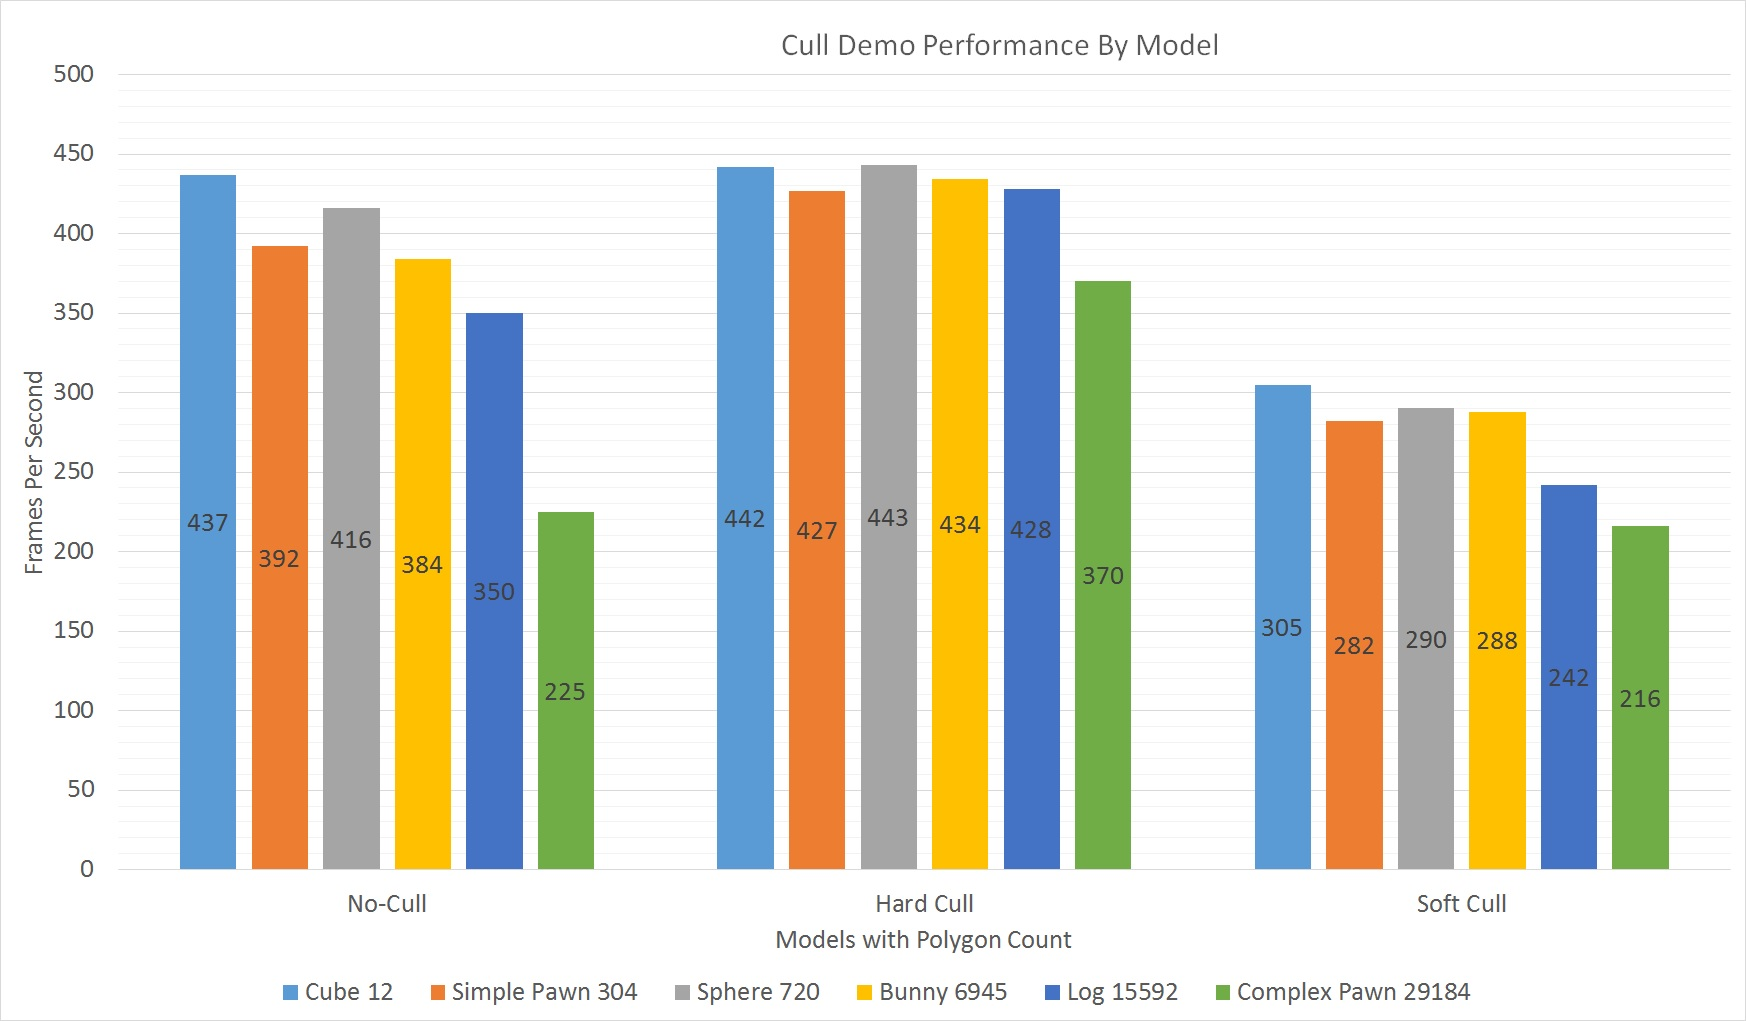
\includegraphics[width=1.0\textwidth]{CDByModel.jpg}
	\caption{Cluster Bar Visualization of Framerates, Sorted by Model}
	\label{pic:CDByModel}
\end{figure}

\noindent \\ There was an interesting trend between the No-Cull mode and the
Software Cull mode, as well. The comparison between these two modes is key, as
the Hardware culling mode does not pass all polygons and potential pixels
through to the pixel shader stage, and these other two modes do. To get an
idea of the raw toll of which pixel Synchronization takes, the results of
these two modes were compared. In figure \ref{pic:CDFrameDiff}, the raw
difference in framerate is shown, not a percentage. As can be seen, the actual
numbered difference in frames varies only slightly, until a model much larger
than the others is used. Then, the difference drops significantly. When
compared with the Framerate output values given in figure \ref{pic:CDGraph},
it can be concluded that Pixel Synchronization hinders performance with
decreasing significance as the primitive assembly stage becomes more of the
bottleneck. In other words, the more vertices the GPU has to process, the
smaller the performance hit incurred by Pixel Synchronization. This conclusion
can be further corroborated by examining \ref{pic:CDPercentGraph}. At first
glance, this plot follows the same pattern as figure \ref{pic:CDFrameDiff}.
However, this shows that the percentage of performance hit that is incurred
decreases with model size. It is up to the programmer to make informed
decisions about the size of models on which to run pixel synchronization.
However, for culling, it is recommended that hardware culling be used wherever
possible, unless the goal is to use pixel synchronization on a single-pass. 

\begin{figure}[!htb]
	\centering
	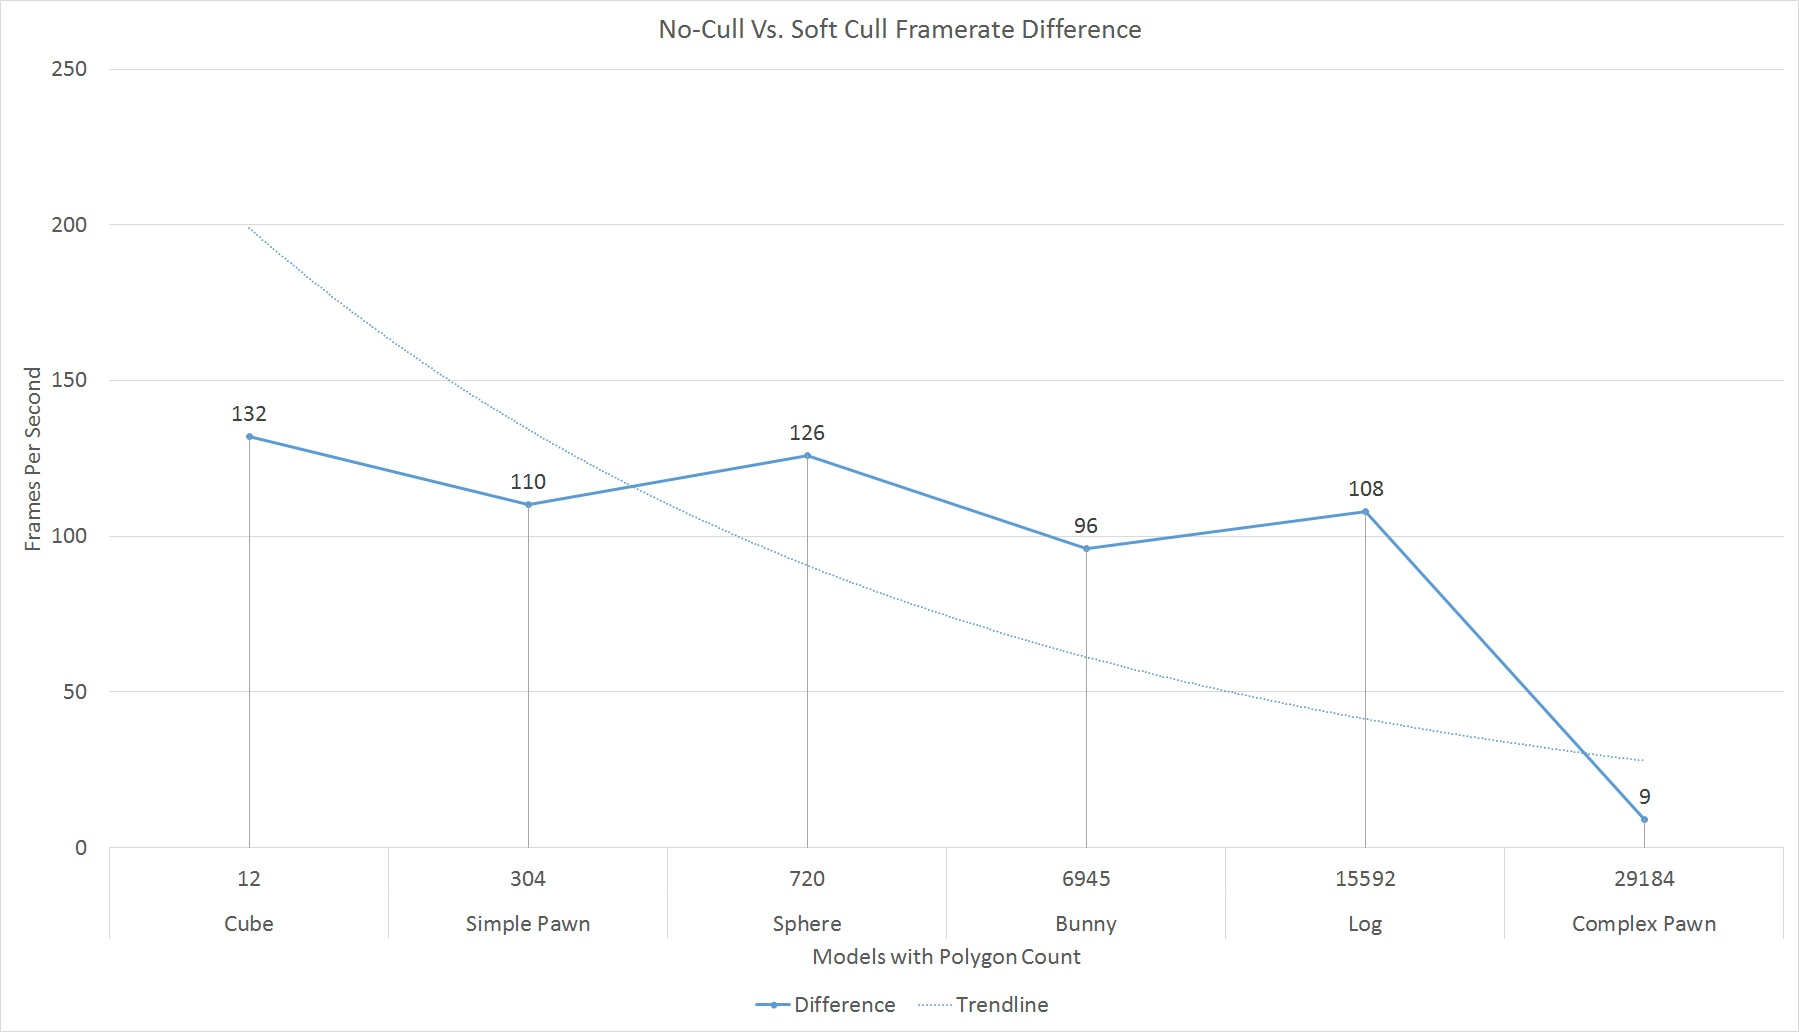
\includegraphics[width=1.0\textwidth]{CullDemoFrameDifference.jpg}
	\caption{Plot of Differences of No-Cull Vs. Soft Cull Framerates}
	\label{pic:CDFrameDiff}
\end{figure}

\begin{figure}[!htb]
	\centering
	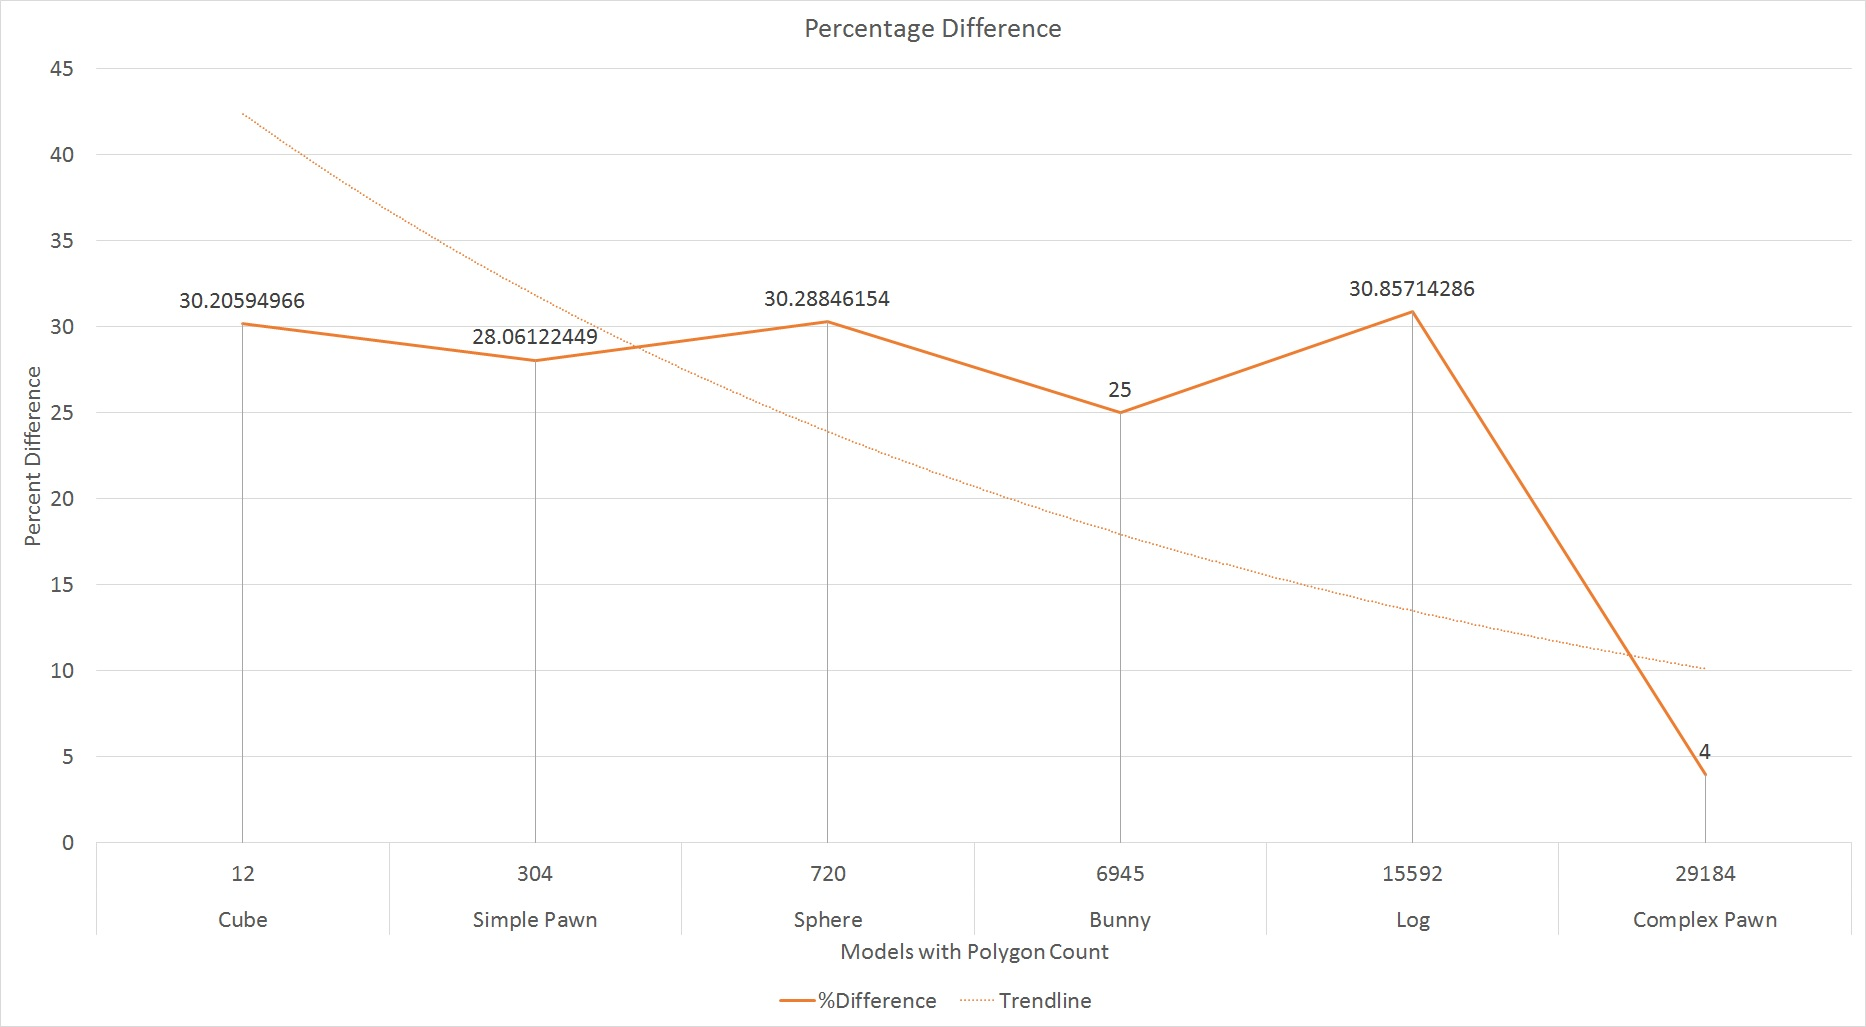
\includegraphics[width=1.0\textwidth]{CDPercentGraph.jpg}
	\caption{Plot of Differences of No-Cull Vs. Soft Cull Framerates}
	\label{pic:CDPercentGraph}
\end{figure}

\subsubsection{Subsurface Scattering}

The results from figure \ref{pic:SSSGraph} are just as expected, with Phong
illumination winning out, performance wise. However, the performance of the
Subsurface Scattering technique is high enough that it would be a viable
technique for use, as it does not tax the GPU so much as to drop the
performance to a less-than desirable frame rate. For increased image quality,
it can be safely concluded that pixel synchronization can help in
accomplishing straightforward solutions to depth-based rendering techniques.

\begin{figure}[!htb]
	\centering
	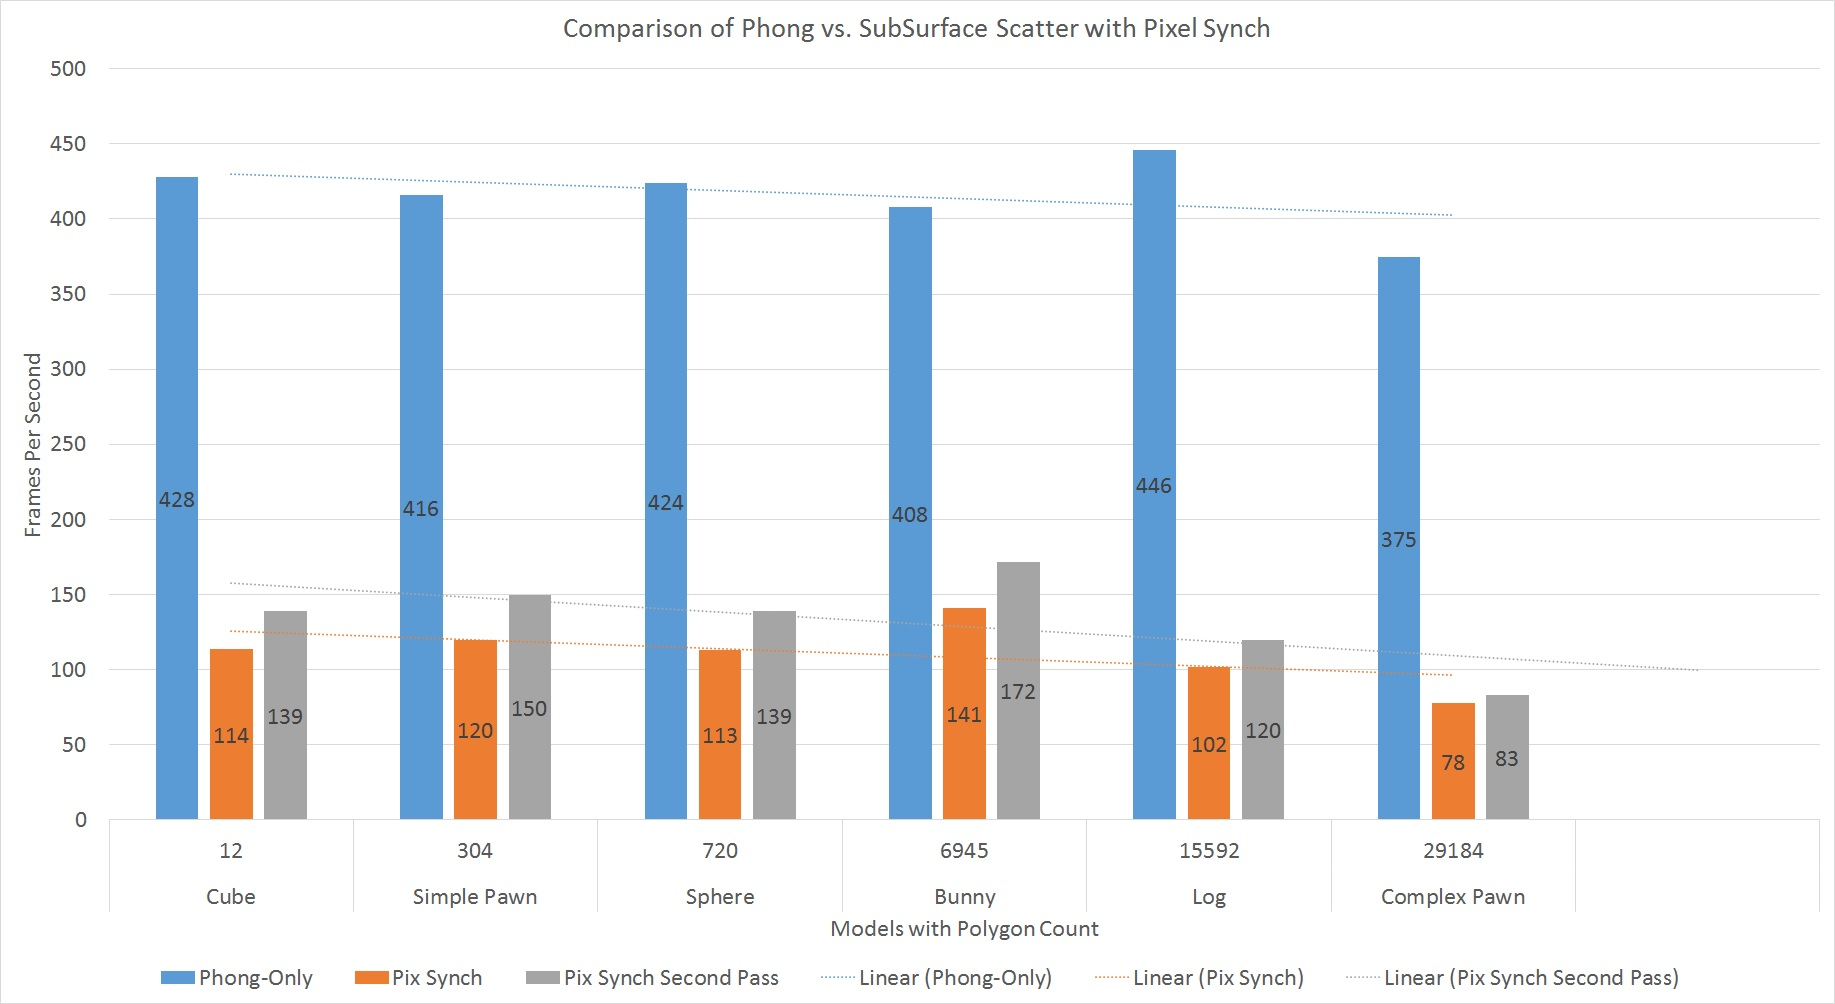
\includegraphics[width=1.0\textwidth]{SSSGraph.jpg}
	\caption{difference between the regular 1-pass phong illumination, timing of 2nd and 3rd passes of pixel synch SSS technique}
	\label{pic:SSSGraph}
\end{figure}

\noindent  Figure ref{pic:SSSPerTechnique} shows an interesting phenomenon.
Consider the left group of the bar graph. The pattern of the leftmost three
members is the same as it has been throughout the other parts of the demo.
However, on the right grouping, the pattern is flipped. One hypothesis that
was devised and tested (results in figure \ref{pic:SSSOrthoSize}) was that it
was the size of the screen space that was taken up by the orthogonal pixel
synchronization step was where the pawn model gained a performance advantage
over the other two models in question. However, as can be seen within figure
\ref{pic:SSSOrthoSize}, this does not end up being the case. This suggested
that the bottleneck could be happening during the first pass, where the models
are unwrapped with respect to texture space, which led to a new hypothesis
that the more texture coordinates that were covered by the model, higher the
performance hit, as the information gathering and storing process takes
longer, as more indices of the texture space are being accessed.

\begin{figure}[!htb]
	\centering
	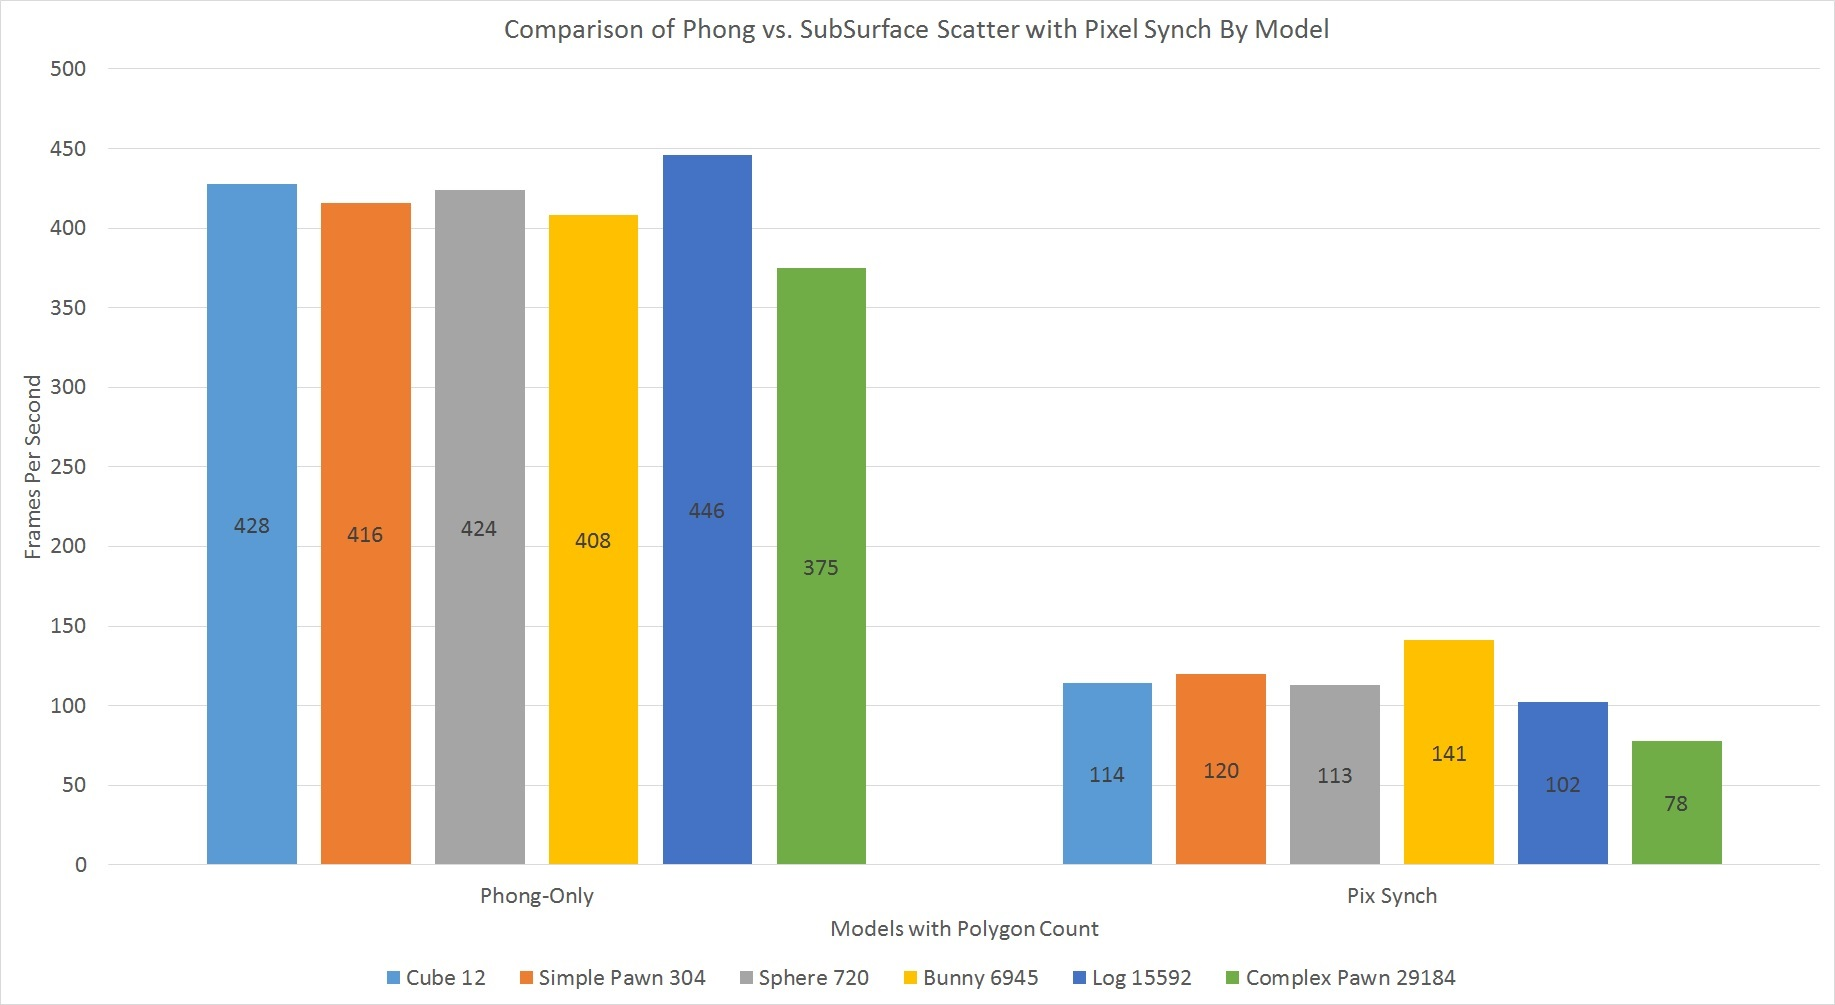
\includegraphics[width=1.0\textwidth]{SSSPerTechnique.jpg}
	\caption{each model's performance, grouped by technique}
	\label{pic:SSSPerTechnique}
\end{figure}

\begin{figure}[!htb]
	\centering
	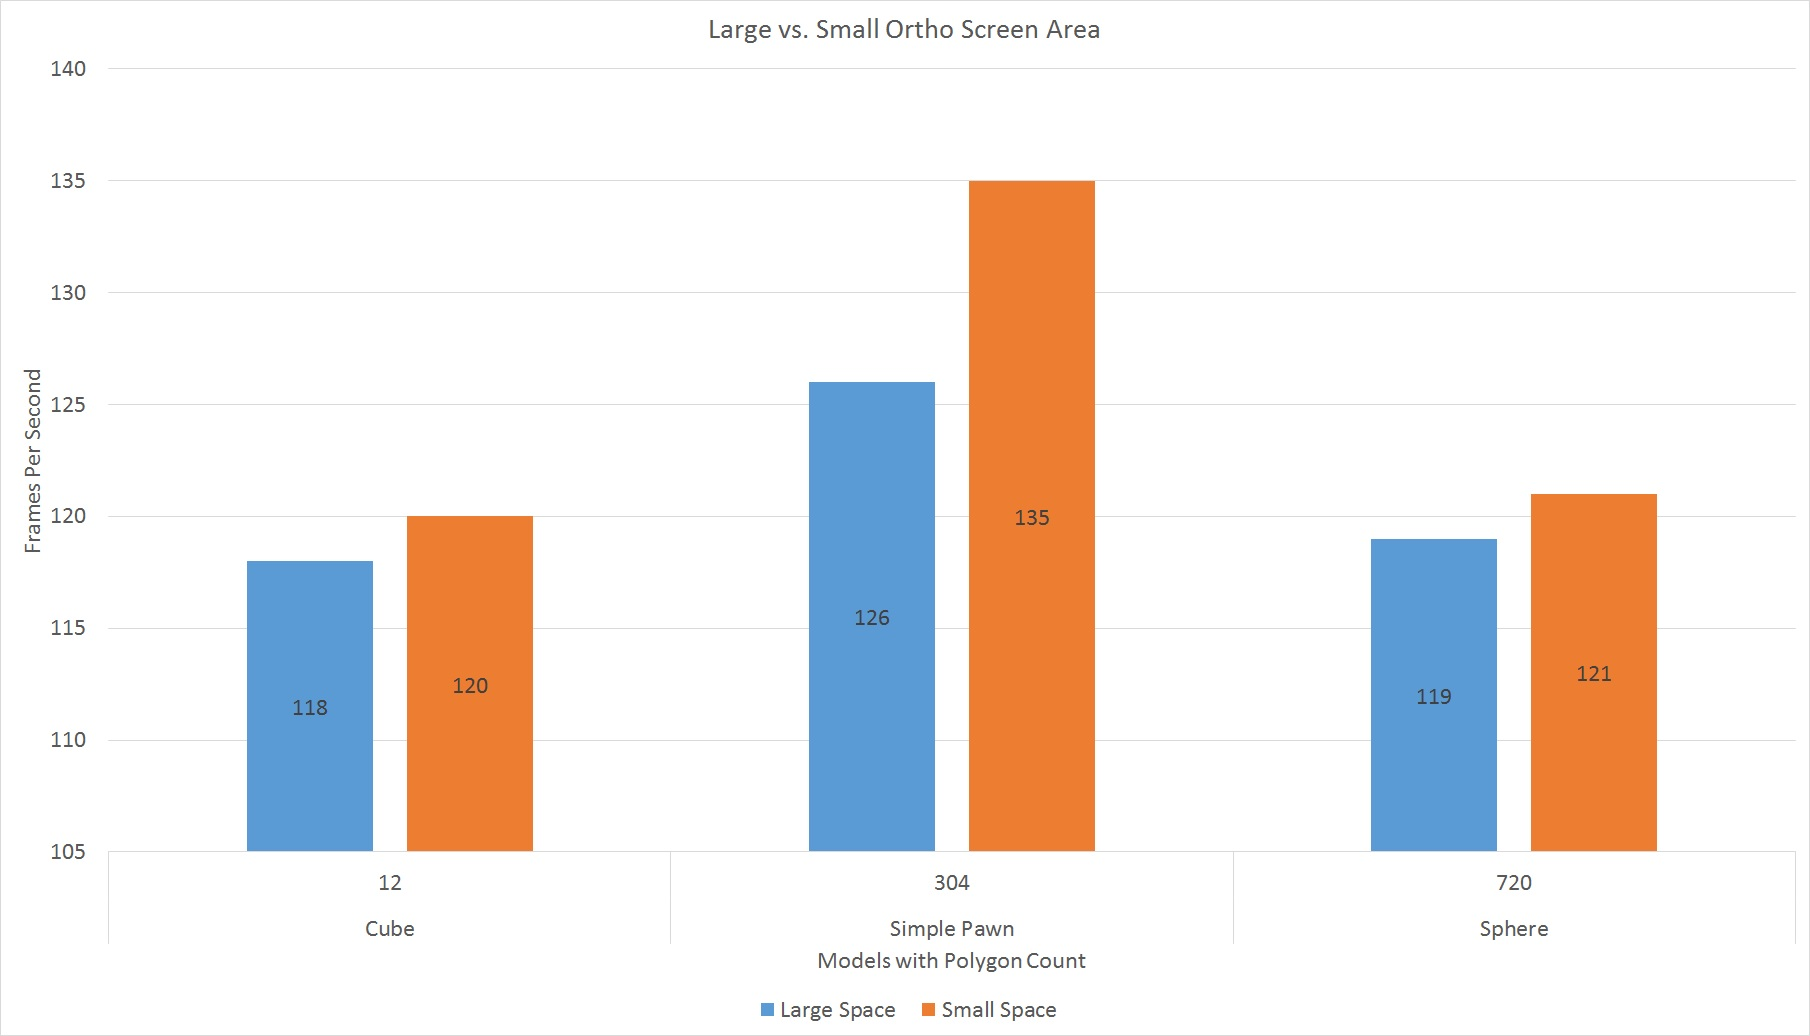
\includegraphics[width=1.0\textwidth]{SSSOrthoSize.jpg}
	\caption{Comparison of screen space taken up by model in pixel synchronization step}
	\label{pic:SSSOrthoSize}
\end{figure}

\noindent   Consider figures \ref{pic:pawnSpace}, \ref{pic:sphereSpace} and
\ref{pic:cubeTSpace}. As can be seen, the pawn's texture space takes up the
least screen space in the first pass. Further, regardless of the number of
vertices within the model, the more pixels that are in flight, the longer a
render pass will take to complete. This conclusion can be corroborated with
the graph in figure \ref{pic:Pass1Graph}. The amount of gray space (pixels
never dispatched) seems to correlate with the performance results. As such, it
is safe to conclude that the bottleneck for models with sufficiently low
vertex counts seems to be the first pass for gathering depth and screen space
knowledge, from the perspective of the light source.

\begin{figure}[!htb]
	\centering
	\includegraphics[width=1.0\textwidth]{pawnSpace2.jpg}
	\caption{Texture space rendering of low-res pawn model}
	\label{pic:pawnSpace}
\end{figure}

\begin{figure}[!htb]
	\centering
	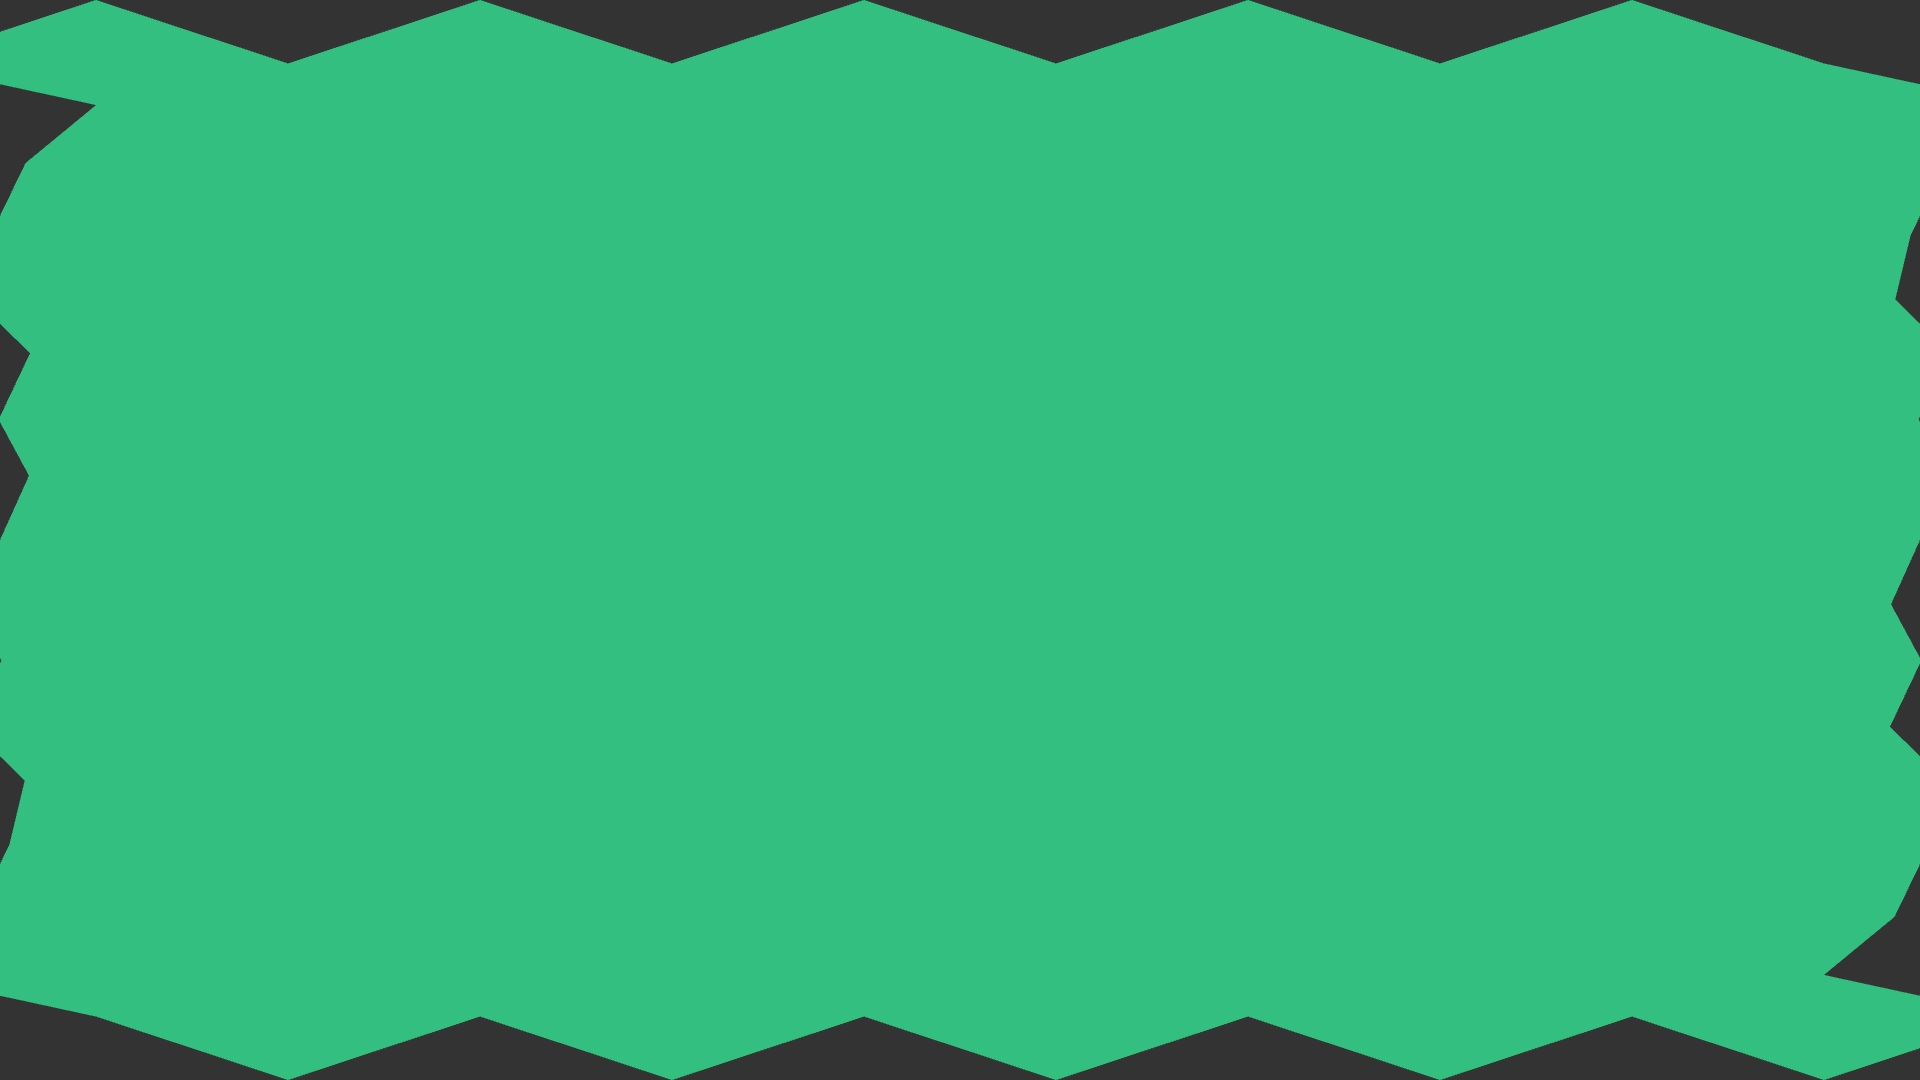
\includegraphics[width=1.0\textwidth]{sphereSpace.jpg}
	\caption{Texture space rendering of sphere}
	\label{pic:sphereSpace}
\end{figure}

\begin{figure}[!htb]
	\centering
	
\includegraphics[width=1.0\textwidth]{cubeTSpace.jpg}
	\caption{Texture space rendering of cube}
	\label{pic:cubeTSpace}
\end{figure}

\begin{figure}[!htb]
	\centering
	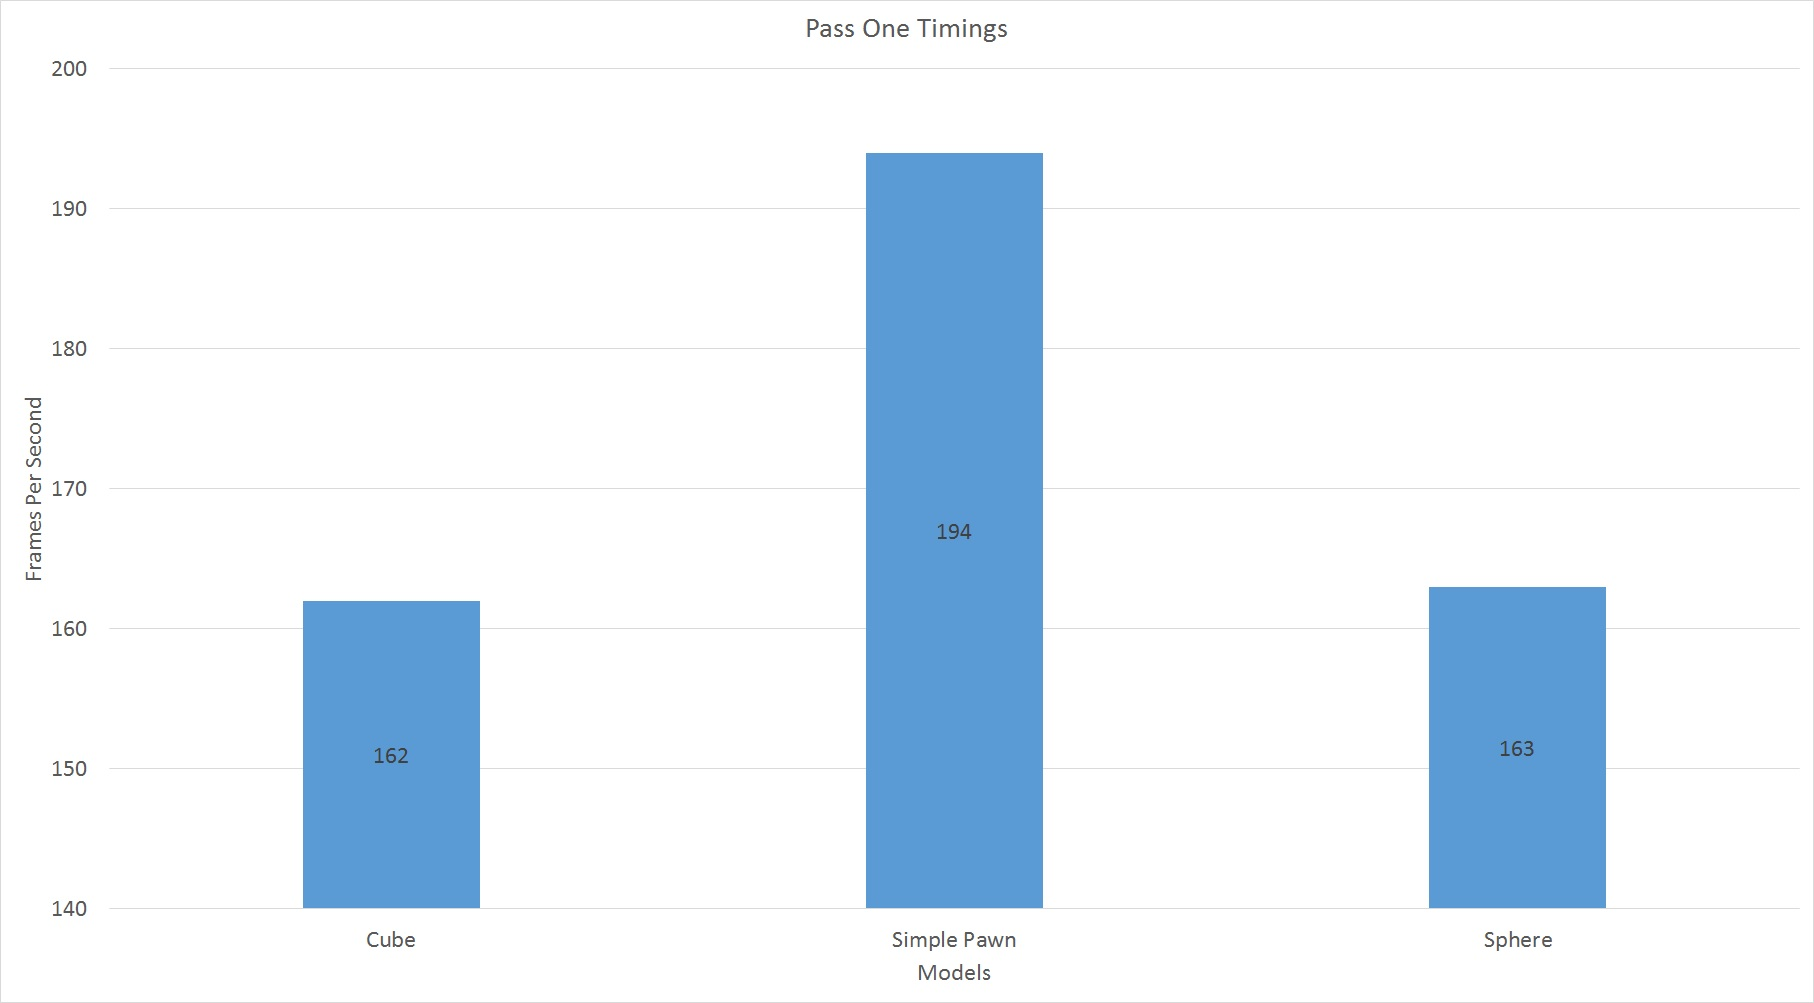
\includegraphics[width=1.0\textwidth]{Pass1Graph.jpg}
	\caption{Texture space render performance}
	\label{pic:Pass1Graph}
\end{figure}

\subsubsection{Refraction}

The attempt at utilizing pixel synchronization to accomplish refraction was
not successful. This being the case, there are no graphs or comparisons of
performance for this portion. However, a formal definition of the algorithm
will be provided, such as to give a hypothetical evaluation on performance
costs with comparison to the simple solution to refraction. \\ \\ From a
high-level perspective, the simple refraction algorithm can be defined in two
steps. These steps assume that the skybox, or cube map, has already been
processed and rendered, and the steps below take place for each pixel.

\begin{description}

\item[Step 1:] calculate the bounce of the eye's ray against the surface
normal.

\item[Step 2:] map the direction of this bounce to a location of the
environment texture.

\end{description}

\noindent With such a simple set of steps, it can be said that for each pixel,
this algorithm runs in constant time, O(1), as it has no other dependencies
upon other pixels, or tracing over another data structure. With this simple
implementation in mind, consider the following steps for the more accurate
refraction approximation. There are two render passes within this method:

\begin{description}

\item[Render Pass 1:] \hfill

\begin{description} 

\item[Step 1:] Store surface normal at the object's location within a 3D
texture that encases the entire view volume.

\item[Step 2:] Mark current location to indicate it is at the surface of the
model. Mark all subsequent locations in the Z direction to indicate that they
are either inside of outside of the model (explained in figure
\ref{code:VoxMask}).

\end{description}

\item[Render Pass 2:] \hfill

\begin{description}

\item[Step 1:] Calculate ray bounce relative to pixel's surface normal.

\item[Step 2:] Trace through the scene while within the object in the unit direction of the ray bounce, until the surface is found again.

\item[Step 3:] Calculate additional ray bounce.

\item[Step 4:] Sample environment texture from resulting bounce.

\end{description}

\end{description}

\noindent Considering the first pass only, Step 2 requires that each pixel
step through a texture. In this case, it is assumed that the texture is
N\textsuperscript{3} in size. This means that in the worst case, each pixel
would take linear, O(N), time to complete its execution. Render Pass 2 is more
complex than the first, as there is more than just data gathering happening at
this point in the algorithm. In Step 2, the gathered data is traversed in the
unit direction of the ray bounce. this being the case, the ray now moves in
the x, y an z directions. However, even though this could be 3N time, it is
simplified to general linear, O(N), time. Overall, the total runtime can be
expressed as follows:

\begin{equation}
Total Render Time = RenderCall + O(N) + RenderCall + O(N)
\end{equation}

\noindent \\ Within grahpics, even linear time algorithms can be quite costly
to performance, as this linear run time applies to every pixel within the
pipeline. What this equation translates to, basically, is that were this
algorithm were to be implemented, the designer of the implementation must make
a careful hardware-specific decision about how large the texture should be to
acheive an optimum balance between performance and image quality.

\section{Observations}

\subsection{Creating and Using Unordered Access Views}
\label{section:UAVs}

When using pixel synchronization, Unordered Access Views (UAVs) are key to
allowing a programmer to get all he or she can out of the pixel synch
capability. UAVs are set up to use on the application side, and can be used on
the GPU side after certain specifications are made. Firstly, we must create
and define the UAV on the application side of our program. \\ \\ We first
create a texture for our UAV on the application side. To create our texture,
we have to create a description to send to the system, then create a texture
by that description (fig. \ref{code:texDesc}). Notice in the code on line 10,
we populate a member of \textbf{texDesc} called \textbf{BindFlags}, and
specify that this texture will be used for unordered access. The population of
this flag does not mean the UAV will be set up and ready for use. \\ \\ We
must map a UAV instance to that texture (fig. \ref{code:mapUAVtoTex}). We must
first describe the instance of the UAV to the program. We do this in a very
similar way to how we described our texture. However the description structure
is now of type \textbf{D3D11\_UNORDERED\_ACCESS\_VIEW\_DESC} instead of
\textbf{D3D11\_TEXTURE2D\_DESC}. As a quick note, the texture description can
be interchangeable among \textbf{D3D11\_TEXTURE1D\_DESC},
\textbf{D3D11\_TEXTURE2D\_DESC} or \textbf{D3D11\_TEXTURE3D\_DESC}\; you must
make sure that the dimension of the UAV description matches what you have
described and created for your texture. If no error occurs after executing the
code in figure \ref{code:mapUAVtoTex}, then we are only a couple of small, yet
key, steps to utilizing UAVs within our code.

\begin{figure}[h]
\begin{lstlisting}[language=C++,breaklines=true]
D3D11_TEXTURE2D_DESC texDesc;
ZeroMemory(&texDesc, sizeof(texDesc));
texDesc.Width = SCREEN_WIDTH;
texDesc.Height = SCREEN_HEIGHT;
texDesc.MipLevels = 1;
texDesc.ArraySize = 1;
texDesc.SampleDesc.Count = 1;
texDesc.SampleDesc.Quality = 0;
texDesc.Usage = D3D11_USAGE_DEFAULT;
texDesc.BindFlags = D3D11_BIND_UNORDERED_ACCESS;
texDesc.Format = DXGI_FORMAT_R32_FLOAT;

//We then use our description to create our texture.

HRESULT texRes = dev->CreateTexture2D(&texDesc, NULL, &pUAVTex);

//We always have a hook to check if our 
//device-side calls were successful.
if (texRes != S_OK)
{
	MessageBox(HWND_DESKTOP, 
		  L"Texture Creation Unsuccessful!", 
		  L"Texture Error!", MB_OK);
	exit(EXIT_FAILURE);
}

\end{lstlisting}
\caption{Describing and creating the 2D texture that we will use for our UAV.}
\label{code:texDesc}
\end{figure}

%-----------------------------------------------------------------------------

\begin{figure}[h]
\begin{lstlisting}[language=C++]
D3D11_UNORDERED_ACCESS_VIEW_DESC UAVdesc;
ZeroMemory(&UAVdesc, sizeof(UAVdesc));

UAVdesc.Format = DXGI_FORMAT_R32_FLOAT;
UAVdesc.ViewDimension = D3D11_UAV_DIMENSION_TEXTURE2D;
UAVdesc.Texture2D.MipSlice = 0;

HRESULT UAVRes = 
	dev->CreateUnorderedAccessView(pUAVTex, 
		&UAVdesc, &pUAV[1]);

if (UAVRes != S_OK){
	MessageBox(HWND_DESKTOP, 
		L"Our UAV view was not successful...", 
		L"UAV Error!", MB_OK);
	exit(EXIT_FAILURE);
}
\end{lstlisting}
\caption{Mapping our UAV to the texture we created in figure \ref{code:texDesc}}
\label{code:mapUAVtoTex}
\end{figure}

\noindent \\ Now that we have a texture created, and a UAV instance bound
to that texture, we must now tell the GPU when we want to utilize the UAV and
where exactly we want that UAV to be mapped, register wise, on the GPU side.
We do this by making a call to the GPU to not only set the render target, but
also the UAVs tied to this render pass. So, we change the set render target
call, as shown in figure \ref{code:setRTV}.

\begin{figure}[h]
\begin{lstlisting}[language=C++]
//we change from this call...
devcon->OMSetRenderTargets(
		numTargets, 
		&RenderTargetViews, 
		DepthBuffer);

//...to this call...
devcon->OMSetRenderTargetsAndUnorderedAccessViews(
		numTargets,
		&RenderTargetViews,
		DepthBuffer,
		UAVStartSlot,
		NumUAVS,
		&UAVs,
		UAVInitialCounts);
\end{lstlisting}
\caption{Comparison of the two OMSetRenderTargets*() calls.}
\label{code:setRTV}
\end{figure}

\noindent \\ After we change this call, we know exactly in which registers
our UAVs will live. So, following that, we make sure to specify where these
UAVs live on the shader side as a global variable, as shown in figure
\ref{code:UAVShaderSide}. A few things to note: In the code, The token
"DataType" should be replaced with whatever datatype was specified
(\textbf{unsigned int}, \textbf{float*}). Something to consider, though, is
that each element within a UAV texture is limited to 32 bits. I recommend
\textbf{float3} only be used in very specific cases, where precision is not
paramount, as you are only able to specify a format of
DXGI\_FORMAT\_R11G11B10\_FLOAT, which means that a programmer is only given 11
bits for the first and second channels, and 10 bits for the third channel.
There are special registers in HLSL shaders in which we must utilize for the
use of UAVs. There are 8 of these registers, and they are preceded with a
'u'. By specifying our register, we know exactly what the datatype and
makeup of that UAV is, by what we have defined on the application side.

\begin{figure}[h]
\begin{lstlisting}[language=HLSL]
RWTextureXD<[DataType]> UAVName : register(uY);
\end{lstlisting}
\caption{General layout of UAV declaration on the shader side Where \textbf{X} is a dimension from 1 to 3, and \textbf{Y} is a register number from 0 to 7. }
\label{code:UAVShaderSide}
\end{figure}

\noindent \\ To reiterate, a UAV is a texture that has been mapped to a
read/write register on the GPU. Since it is a texture, we can also sample from
it. This behavior exists for the following reason: say we populate this UAV
texture in one shader pass, then want to read from it within a different one.
This can be accomplished in two ways, but some programmers prefer to sample
from the texture using the sample intrinsic, rather than indexing it like a
UAV. To do so, we would have to specify that we want our texture to be used as
both a UAV and a read-in texture, by changing the bind flags from
\textbf{D3D11\_BIND\_UNORDERED\_ACCESS} to
\textbf{D3D11\_BIND\_UNORDERED\_ACCESS $|$ D3D11\_BIND\_SHADER\_RESOURCE}.
This allows us to also tie a texture sampler to the same texture that a UAV is
bound to. However, to smaple from the texture, we must firt unplug it from the
program as a UAV and plug it back in as a sampled texture. This means that
writing to a texture, then sampling from it in the same pass would not be
allowed (nor would it be very practical). A good use for setting a texture as
both a UAV and a Sampled Texture would be in a case such as the Subsurface
Scattering demo, where we store the depth of each fragment, with respect to
the light in one pass, as well as which ray passes through that fragment.

\subsection{Unordered Access View Limitations and Recommendations}

\label{section:UAVLimits}

UAVs are quite useful in the grand scheme of things, but how useful they can
be, really depends on the amount of memory the GPU has at its disposal, and
whether or not the data the programmer would like to store must be iterated
over. The memory bandwidth issue is not necessarily a pressing one for the
demo presented within this paper, but it could present itself as an issue for
larger projects, if not monitered. \\ \\ UAVs cannot be looped over within a
shader. What this means, is that if a programmer would like to search for a
value within a UAV, this is not possible and the HLSL compiler will not even
compile the programmer's shader. This means that any sort of iteration over
dynamic data within a pixel shader is not possible at this time. I speculate
that this is done as a precaution to keep programmers from shooting themselves
in the foot, or creating an infinite loop within the GPU, which could cause
trouble in the form of Denial of Service. However, if the programmer sets up
their UAV diligently within the shader, this should never be the case. \\ \\
Another issue is that application side UAVs and their Shader-side counterparts
are seemingly very disparate entities within code. A programmer must be very
diligent in keeping track which UAVs are tied to which textures, what datatype
is associated with said UAV, whether or not the UAV is bound, and if bound, to
which register. However, following all of the bookkeeping steps, UAVs make
shaders more powerful. \\ \\ As mentioned above, there are 8 UAV registers
available on the hardware on which I ran my code. However, we may only bind 7
UAVs at a time, since one of these UAV registers is actually reserved for the
render target (if we are utilizing UAVs within a pass that renders to screen).
When designing a graphics program, remember to keep track of how many
Read/Write datastructures needed within the GPU, and which can be sampled as
textures at any point. It is also recommended that a programmer become very
familiar with data packing algorithms, such that the 32 bits per each UAV
element is used to as much of its capacity as possible. Packing data
efficiently will lead to a far more efficient HLSL program, as long as the
pack/unpack functions are quick. \\ \\ There remain other issues while using
UAVs, including the following:

\begin{description}

\item[Clearing UAVs] \hfill \\ 

Clearing a UAV on the application side can be quite expensive, and seems to
scale quite a bit with the size of the UAV. For instance, within my refract
code, I have a UAV that points to a Texture3D that greatly slows down the
performance of the application. Please see figure (make figure) for a visual
explanation. It is up to the programmer's discression to discern a 'sweet
spot' size for their UAVs to get equal parts quality and performance. As can
be seen in the graph, having a large UAV can really slow down a render pass.

\item[Uninitialized UAVs] \hfill \\

Within HLSL code, the compiler allows the programmer to define a RWTextureXD,
as demonstrated in figure \ref{code:UAVShaderSide}, at any time. There is no
check from the compiler to see if there is a UAV register that has been
initialized to a texture. The reason why is because shader programs are
compiled and linked prior to setting any UAVs. In other words, the HLSL
compiler allows this because it is trusting the programmer to populate that
register with a texture when it comes time to run the shader program. However,
if a UAV is never initialized or populated, the programmer may still reference
that RWTexture, but any writes to or reads from will not work. In most cases,
any read or write will cause the program to crash. Any methods specific to
RWTexture can still be executed, such as RWTexture2D.GetDimensions(). However,
the X and Y dimensions returned will just be zero. This is an easily avoidable
pitfall, so long as the programmer keeps track of his or her UAVs accordingly.

\item[UAV Order is important] \hfill \\

Programmers using UAVs in their shader code must keep track of the order in
which their they are given to the GPU when Binding their UAVs and Render
Target(s). Seeing as this is only possible if the UAVs are kept in an array,
it is good to keep a note of which UAVs are meant for certain purposes. If
multiple sets of UAVs are needed, it is recommended these UAV sets are named
accordingly. While rendering, shader code is allowed to access UAVs as a
datatype that conflicts with what a programmer might have defined at that UAV
slot, because every element in a UAV texture is 32 bits. This makes it quite
difficult to catch potential errors, unless diligent precautionary measures
are taken.

\end{description}

\subsection{Pixel Synchronization Behavior}

\label{section:PSBehavior}

The Behavior of Pixel Synchronization can be confusing, unless if we take time
to understand what it actually does. However, let us first take the time to
figure out how prepare it for use on the application side. In order to see if
the Iris extensions are available, the programmer must include the following
files into his or her C++ code: \textit{ID3D10Extensions.h},
\textit{IGFXExtensionsHelper.h} and \textit{IGFXExtensionHelper.cpp}. These
three files can be found within the github repository in the IGFXExtensions
folder. After including these files in your C++ application, the programmer
may now use the IGFX namespace. To initialize these extensions, simply execute
the following commands during the DirectX setup function (in this project,
this part of code is called \textbf{InitD3D()}). As is shown in figure
\ref{code:extInit}, to initialize Iris Extensions on the application is quite
simple. This is because Iris Extensions are meant to happen without having to
be too visible to the DirectX side of code. After we initialize our graphics
extensions, we can see which extensions we have available to us, if any. Now
that we have this information, our program can make informed decisions on what
kind of hardware it has at its disposal to accomplish render techniques. As
this demo is meant only for Iris extensions, a decision was made to not
utilize this available extension check to enhance robustness of the program.

\begin{figure}[h]
\begin{lstlisting}
//global variable...
IGFX::Extensions myExtensions;

//Within setup code...
HRESULT res = IGFX::Init(dev);
if(res == S_OK) myExtensions = 
	IGFX::getAvailableExtensions(dev);

\end{lstlisting}
\caption{Intel Iris extension setup on the application side.}
\label{code:extInit}
\end{figure}

\noindent \\ After we ensure our program/Direct3D device  can use Pixel
Synchronization, there isn't anything more that the GPU device requires from
the application, itself. Now, all we must do is specify when, inside of our
pixel shader, we want to synchronize our pixels, and that's it! For an actual
shader code snippet of this, please refer to the snippet in section
\ref{section:PixSyncIntro}, figure \ref{code:PSExample}. Recall that the Pixel
Shader must include \textit{IntelExtensions.hlsl}. \\ \\ So at this point, we
should be able to initialize Iris Extensions and invoke Pixel Synchronization.
However, as programmers, we can't very well utilize Pixel Synchronization
without first knowing how it behaves. \\ \\ When invoked, it is known that
Pixel Synchronization first creates a barrier for all shaders in flight at the
same pixel position. Following this barrier, we know that all shaders that hit
this barrier are ordered by Primitive ID. The question is, "How does this
ordering occur?" The answer is actually quite straightforward. They appear to
be ordered by primitive number because they are ordered by order of submission
from the vertex stage. Knowing that this happens, whether the pixels actually
accomplish a front-back or back-front sorting depends on how the model was
defined within its object file. \\ \\ Knowing that the ordering takes place as
such, it is not safe to assume that the ordering will take place the way the
programmer wants to. As a result, this begs the question: What is the benefit
of Pixel Synchronization, exactly? The benefit of this extension comes from
the fact that we can guarantee a portion of memory will be read/written
without data races. This allows for programmers to accomplish much more within
the pixel shader than has been done before. To be able to accomplish sorting
based upon depth within the shader is a remarkable thing. However, there are
some workarounds that must take place. As it was mentioned in section
\ref{section:UAVLimits}, we cannot loop over our UAVs, but one thing we are
able to do is make create a 'mask' that keeps track of what depth of a
Texture3D or Texture2D array has not been written to, then write to that.
After this step, we can sort through the UAV as a sampled texture in a later
pass, such that we can do something meaningful with the information.

\subsection{Coding and Behavior Quirks}

As this project deals with raw DirectX, there are a lot of places in code
which could serve as confusing pitfalls. These pieces of code range from
application or CPU-side issues, or even within the pipeline itself. This
section is meant to detail some of those more common pitfalls and also point
out some behavior inherent to the pipeline or hardware that are not the
programmer's fault.

\subsubsection{Working With the GPU Device on the Application Side}

Just the same as in OpenGL applications, DirectX applications allow the
program to continue even if there is an error or failure within the graphics
device. For this reason, self-error checking is a very important practice when
building a graphics program from scratch. Within a DirectX application, this
can be easily done, as the appropriate device and device context related
functions return a datatype called HRESULT. By checking this HRESULT, a
programmer can get a good idea of what type of error is happening within his
or her code. However, this doesn't encompass all errors. There are some
instances in which a call to the GPU can cause an internal error, and force
the device to unplug itself from the program. The instance in which this
"Device Removed Error" occurred most commonly for this project was when
attempting to create a UAV texture that was too large for the program. If the
program is allowed to let itself run without having this error caught, other
errors will occur down the line, and in the best case, the program will yield
a viewport full of garbage.

\subsubsection{Pipeline Behavior}

The most fascinating behavior of the pipeline during this project was finding
that the pipeline may make rounding errors during the interpolation phase of
the pipeline. These rounding errors were made apparent when attempting to work
with a UAV that was a larger resolution than 512x512 pixels in the Subsurface
Scattering Demo. If the texture was too high of a resolution, the resulting
depth-based shadow would cause an immense amount of artifacts. This was
mitigated when using a lower resolution texture. The only conclusion I could
draw from this was that there were rounding errors taking place within the
interpolation stage, forcing certain indices of the texture to be missed.
Screenshots and a graph demonstrating this behavior can be found on page(put
pictures into this document now, ok thanks).

\subsubsection{Placement of Pixel Synchronization call}

As state previously, making a call to pixel synchronization creates a critical
section within a pixel shader. The catch to this, however, is that, beginning
with the pixel synchronization call, the rest of the pixel shader is a
critical section until the end of the shader. Since this is the case, it is
highly recommended that all operations that are not dependant upon
synchronization happen prior to the barrier to mitigate the number of
operations that must be ordered. However, if the pixel shader does not have
many operations taking place, it may not be a noticeable difference to have
the non-dependant code within the critical section. Code with pixel
syncronization saw a 10\% drop in frames per second, compared to the same code
with the barrier removed.

\subsubsection{Vertices are Still the Bottleneck}

As the vertices have been processed and all values have been interpolated
across the pipeline at the point of the Pixel Shader, a bigger influence on
runtime will still be the number of vertices used to define the 3D object. For
instance, this project contains two pawn models. One is very low resolution
with a smal number of faces, and the other has been smoothed and vertices have
been added. The runtime still scales with the number of vertices, regardless
of any influence of pixel synchronization.

\subsection{Suggestions and Advice When Using Pixel Synchronization}
\label{section:suggestions}

Pixel Synchronization melds the world of graphics and parallelism even
further, by adding the capabilites of barriers to the end of the graphics
pipeline. However, to take advantage of this capability to the fullest, some
practices in parallel programming must be taken up within graphics
programming.

\begin{description}

\item[Design the Critical Section] \hfill \\

Since our critical section will be ordered and will execute one-at-a-time, the
programmer must do what he or she can to keep that section of code lean. To
make sure our critical section is as lean as possible, it is recommended that
the programmer evaluate and design the pixel shader to make smart, informed
decisions on what operations can happen outside or inside of the ordered
section of code. One very simple rule is that any write to or read from shared
memory must take place within a critical section. As a translation, any access
to memory that would require a mutex in a parallel program should be accessed
inside of the Pixel Sync critical section.

\item[Know the Necessary Relationships] \hfill \\

Having multiple render passes per object in a scene is quite costly. However,
a good way to mitigate erroneous passes is to think about the relationship
between the object and, in the case of Subsurface Scattering, the light
source. In the case of Subsurface scattering, we know that the depth
information stored at that object does not change until either the object or
the light changes their orientation within the scene. A flag can be inserted
into the program such that if either of the two involved entities change their
orientation or position, the Pixel Ordering passes are activated to gather the
new depth information. Executing Pixel Ordering passes based upon a condition
has the potential to vastly speed up the runtime of a graphics progrom that
uses this functionality to implement effects such as subsurface scattering,
and help to make a case for its viability in practical use.

\item[Keep the UAVs a reasonable size] \hfill \\

One of the biggest hits to performance was using a UAV texture that was quite
large. UAVs that were large ended up incurring a rather larger performance
hit. To mitigate this, it is recommended to find a "sweet spot" between
quality and performance. Along with the performance of the shaders with the
UAV, it takes quite a bit of time to clear these UAVs with each rendering of
the scene. This was made very apparent when creating a Texture3D UAV of size
$800^3$.

\item[Take Advantage of Having a Texture Be Both a UAV and a Sampled Texture] \hfill \\

Sampling a texture takes less time than indexing a UAV. As this is the case,
it is recommended that the programmer access the texture with a Sampler if the
shader is only reading from the texture, and not Read/Writing. This will help
ensure that the final render pass is as fast as possible.

\end{description}

\subsection{General Suggestions and Advice}

\label{subsection:Suggestions}

When writing raw DirectX, there are some pitfalls and coding tricks that are
necessary to point out. However, paying attention to these pitfalls and tricks
won't necessarily make a programmer's DirectX application bug-free, but
knowledge and consideration of these suggestions and advice could save
debugging and head-scratching time.

\begin{description}

\item[Constant Buffers] \hfill \\

Constant Buffers are how DirectX approaches application-specific variables
within the GPU. For instance, if the programmer would like to include an
interactive coefficient for brightness of a light source, he or she would do
so by creating a constant buffer that held that coeffiecient, then updating it
on the application side prior to rendering. OpenGL approaches this by using
Uniform Variables, all of which have their own ID number on the GPU and are
updated one-by-one. \\ \\ If a programmer has multiple values to pass into his
or her DirectX program, it can be done by adding multiple members to the
constant buffer data structure. This reduces the communication to/from the GPU
to just one instance, while updating the entire buffer. However, it is
important that the definition of the struct on the GPU side mirrors the
application side's definition. Further, take note that the Constant Buffer's
size must be a multiple of 16. This is so the call to copy the information
from the application to GPU will always be a predicatable size for the GPU. To
mitigate problems, the creation of the constant buffer in the Subsurface
Scattering Demo added the size of the constant buffer, mod 16. For a better
idea, please consider the code snippet below. On line 5 in the below code
snippet, the multiple of 16 size constraint is accounted for by adding the
size of the buffer, mod 16. This means that the constant buffer could have
anywhere from 0 to 15 bytes of extra space. Another way to account for the
multiple of 16 size constraint is to add pad variables to the constant buffer,
itself. Some programmers prefer this method, as it gives the padding a
representation in the form of a defined datatype.

\begin{lstlisting}[language=C++]
D3D11_BUFFER_DESC bd;
ZeroMemory(&bd, sizeof(bd));

bd.Usage = D3D11_USAGE_DEFAULT;
bd.ByteWidth = sizeof(CBUFFER) + (sizeof(CBUFFER) % 16);
bd.BindFlags = D3D11_BIND_CONSTANT_BUFFER;

HRESULT bres = dev->CreateBuffer(&bd, NULL, &pCBuffer);

if (bres != S_OK)
{
	MessageBox(HWND_DESKTOP, 
		L"FAILED CONSTANT BUFFER CREATION", 
		L"CBUFFER ERROR", MB_OK);
	exit(EXIT_FAILURE);
}
devcon->VSSetConstantBuffers(0, 1, &pCBuffer);
\end{lstlisting}

\item[Learn the HLSL Semantics] \hfill \\

In HLSL a Semantic is an optional string that identifies the intended usage of
return data. These semantics are quite useful in telling the GPU how to
interpolate values across the pipeline. For instance, consider the following
Data Structure defined in HLSL:

\begin{lstlisting}[language=HLSL, numbers=none, frame=none]
struct VOut
{
	float4 svposition : SV_POSITION;
	float4 color : COLOR;
	float4 position : POSITION;
	float2 UVs : TEXCOORD;
	float4 normal : NORMAL;
	float4 camera : CAMERA;
	float3 lightVec : NORMAL1;
	float4 lightCol : COLOR1;
	uint mode : MODE;
	float4 rotNorm : NORMAL2;
	float3 eyeVec : NORMAL3;
};
\end{lstlisting}

This is a data structure defined within the shader file, such that the vertex
shader can pass many values to the pipeline. Some sematics are built in, but
some others are programmer-defined. In this case, the only programmer-defined
semantic would be MODE. The use for mode will be covered in the implementation
discussion. Notice the differences between the SV\_POSITION and POSITION
semantics. These two Semantics tell the pipeline how to interpolate these
values. As can be seen in the listed Shaders, both the SV\_POSITON and
POSITION members get the same value in the vertex shader. However,
SV\_POSITION gets interpolated into X/Y screen positons, and POSITION gets
interpolated in the same -1 to 1 space for the X/Y/Z position given to it.
Once a fragment or pixel shader has completed its running, the computed color
is assigned to the pixel at the X/Y SV\_POSITION. These semantics are a great
way to keep track of values passed across the pipeline, and helps shed a
little bit more light on what they are, and what they are used for.

\item[Invest Time into Learning a Good Menuing Library] \hfill \\

Creating a menu window for this project could have been made a lot simpler
with a proper menuing library, instead of building it from scratch. The
advantage of using a premade menuing library is that many of the
functionalities of buttons can be linked in a simple call, rather than using
the vanilla window class. For instance, within the Subsurface Scattering code,
the menu was built entirely from scratch, and had to have its own window
process, where it must check the state of global variables with which the
buttons on the menu are tied to, and checked/unchecked, or presed without a
convenient construct for relationship. The problem with this approach is that
the relationship between the menu's buttons and what they are supposed to
indicate, where they are located on the menu window, and which checkboxes are
related to each other all must be managed explicitly by the programmer. In
short, to save time, it is highly recommended that a menuing library be used,
so as to avoid any extra debugging that does not have anything directly to do
with the project.  \\ \\ Further, using the raw windows framework to create a
menu doesn't abstract away anything for the programmer; every bit of the
subclasses that the menu window holds are at the most raw level. For a better idea, please see the code below:

\begin{lstlisting}[language=C++, numbers=none, frame=none]
hGBButton = CreateWindowEx(
	NULL,
	L"BUTTON",
	L"GOOD/BAD",
	WS_TABSTOP | WS_VISIBLE | WS_CHILD | BS_AUTOCHECKBOX,
	50,
	20,
	100,
	24,
	hWnd,
	(HMENU)GOODBAD_BUTTON,
	GetModuleHandle(NULL),
	NULL);

SendMessage(hGBButton,
	WM_SETFONT,
	(WPARAM)hfDefault,
	MAKELPARAM(FALSE, 0));

Button_SetCheck(hGBButton, true);
\end{lstlisting}

To make a button without any menuing library, we must define a new window
instance which lives inside of the current window, $hWnd$, define its size and
position within the window, whether it is a checkbox button, and pass messages
to and from the button, itself. The last line of the listing is meant to show
that the programmer must set whether the checkbox is checked or unchecked,
which implies that the programmer must track the value associated with that
button and change that value accordingly. In short, without a proper Menuing
library, building a menu can become quite convoluted and confusing.

\item[Use Separate Render Functions] \hfill \\

To demonstrate different effects, there could be potentially many differences
in setup and dispatching of the GPU. For instance, the difference between the
regular Phong Illumination technique and the Subsurface Scattering algorithm
utilizing pixel synchronization are quite different, as far as how many UAVs
must be set and bound to the render target and the number of passes. To keep
the code readable and to mitigate too many conditionals within the render
function, it is recommended that each render technique get its own render
function. \\ \\ If render techniques are not separated into different render
functions, there could be mistakes made that could skew timing measurements.
For instance, within the Subsurface Scattering Project, the Phong Illumination
technique had been measured to perform at about the same framerate as the
Pixel Synch Subsurface Scatter. As it turns out, what was happening was that
the two setup render passes were still being executed, then the information
was basically just being ignored. However, problems such as this are specific
to the programmer, and not necesarily a general problem. For readability and
clearcut management of code, splitting render techniques into their own
separate functions is recommended.

\end{description}

\pagebreak

\section{Conclusion and Recommended Future Work}

Coming to conclusions and figuring a roadmap for any potential future work for
a project is almost as important as the project, itself. The following
sections will detail what conclusions this project has presented, as far as
the usefulness and viability of Pixel Synchronization, then potential avenues
for further exploration will be detailed in the latter section. Those ideas
are just to jumpstart the thinking of any student who wishes to undertake a
project using pixel synchronization, and are not the only ideas worth
persuing.

\subsection{Conclusions About the Utility of Pixel Synchronization}

\subsubsection{Key Observations}

Before going into what conclusions were drawn, it is worth detailing the key
observations that took place, as these shaped the conclusions. The following
are a list of observations, and some may be repeats from previous sections of
this paper.

\begin{description}

\item[UAVs limit potential] \hfill \\

The UAV limitation described above in section \ref{section:UAVLimits}. The
restriction of iterating over a UAV is, while understandable, diminishes the
number of algorithms that can potentially be run on a synchronized pixel
shader. As discussed above, this restriction is in place such that the
programmer does not, by either accident or design, put a program onto the GPU
hardware that creates a Denial of Service. Despite this limitation, there are
workarounds, however, such workarounds would add an extra pass to a
programmer's algorithm. For instance, one workaround could be to iterate over
a Sampled texture, then using it as a UAV in the next pass. However, at this
point, the idea of being able to use a UAV is shadowed by the fact that the
programmer would be better off just keeping the texture bound to a sampler and
doing a traditional render to texture and read from texture.

\item[Performance Hit of Pixel Sync Scaled With the Size of the Model.] \hfill \\

As demonstrated in this project, the performance hit scaled as it should have
with the size of the model. This piece of hardware is as unobtrusive to the
original pipeline as it possibly can be, and the size of the model doesn't
affect performance any differently than it used to. Even though the
performance hit scales as it should, that is not to say that it is not
recommended that the programmer choose the critical section wisely. The
smaller the critical section, the fewer the operations that must happen in-
order. If at all possible, the best critical section would be one where only
writes to the UAV take place. However, since most algorithms rely on reads and
writes, this is a very tough case to acheive.

\item[Pixel Synchronization Orders Pixels Based Upon When They Were Submitted] \hfill \\

Seeing as the pixels are ordered based upon submission, and not depth, means
that the programmer must still keep track of which pixels are deeper than
others, when doing any sort of depth-based calculation. However, so long as
the programmer designs the algorithm such that there is a quick check, depth-
based decisions can be made in the same pass rather easily. Such an example of
this is with the software culling example included in the Sub-Surface
Scattering demo.

\item[Pixel Synchronization is a Per-Pixel Mutex] \hfill \\

As stated before, Pixel Synchronization's main purpose is to eliminate race
conditions within Pixel Shaders. As such, Pixel Synchronization is a fantastic
tool for naive calculations such as blending or transparency, since a pixel
need only read/write a single value. Any algorithm that requires a naive
addition or subtraction is already very well set up for the use of Pixel
Synchronization. However, since this inherent mutex is in place, there are
still many interesting solutions to be found within its use. \\ \\ With Pixel
Synchronization, a programmer would be able to write a shadow mapping shader
program with fewer render passes. All that must happen for the depth-based
part of the shadow map is for the pass with respect to the light to mark which
surfaces it can hit. Following that calculation, the render pass shader could
make an informed decision on which parts of objects to illuminate, and which
parts of objects not to illuminate.

\end{description}

\subsection{What the Findings Mean}

Given the findings, there are a number of conclusions we can draw from this
project. We can safely say that Pixel Synch is a great tool for a set of
problems, careful design decisions will help make Pixel Synch algorithms
relatively unobtrusive to runtime, all hardware could benefit from such a
capability, and increased UAV functionality within the shader could unlock
more potential.

\begin{description}

\item[For Certain problems, Pixel Synch is a Great Tool] \hfill \\

Of course, Pixel Synchronization is not the be-all, end-all solution to
increasing a graphics program's efficiency or quality. There are many key
factors that attribute to the amount of utility that Pixel Synchronization
will provide. If a graphics programmer were to be implementing a data-parallel
rendering algorithm, this feature is quite useful. Any sort of depth-based
problem would benefit very much from the use of Pixel Synchronization. In some
cases, it can aid in performance, and in others, it can simply aid in
simplifying the algorithm for readability, or reduce the amount of information
the algorithm needs to run. As for the case of Subsurface Scattering, Pixel
Synchronization was used to increase the quality of the image, and nothing
more. After a small tweak to the Subsurface Scattering algorithm, the program
was able to run at a performance similar to Phong Illumination in some cases.

\item[When designing a Pixel Synch Algorithm, Do So Carefully] \hfill \\

When finding a method of utilizing pixel synchronization for a rendering
algorithm, there are important aspects to keep track of; for example:

\begin{itemize} 

\item How much memory does the GPU have?
\item What size of texture would work for this algorithm?
\item How much of the Pixel Shader must happen after Pixel Synchronization?

\end{itemize}

There are other factors among the above three questions, but those seem to be
the most fundamental and most considered when designing algorithms using Pixel
Synchronization. Throughout the project, the GPU memory size, texture size and
size of the critical section were the main factors within the design. After
finding a "sweet-spot" answer to these questions, the Pixel Synchronization
stage was able to be fit into the rendering algorithm in a way that was
relatively unobtrusive to runtime.

\item[Pixel Synchronization Would Be a Welcome Addition on All Graphics Hardware] \hfill \\

Seeing as Pixel Synchronization has had such an impressive effect on a
CPU/GPU, It seems as though this capability would have great potential on
larger discrete graphics hardware. Since the beginning of this project, this
has become the case for nVidia hardware, with the introduction of nVidia's
"Pixel Interlock" technology. Seeing this concept make the jump to discrete
graphics hardware indicates a promising future for Pixel Synchronization.
However, there must be more exploration and experimentation as far as what
ideas this could lend itself well to.

\item[Trusting the Programmer to Loop Over UAV Textures Will Be Beneficial]
\hfill \\

As previously stated, the HLSL shader compiler does not allow for a loop to
have a condition that depends upon a read from a UAV. This could be a
restriction based upon the fact that Pixel Synchronization is not a widely
used extension and the compiler simply assumes that there will not be ordered
access to the UAV elements. If the compiler were to allow conditionals within
loop constructs which depended on information within the UAV, the potential of
Pixel Synchronization would grow immensely. At the very least, it would be
good for the programmer to be able to set a flag for the HLSL compiler that
says, "trust me, I'm using pixel synchronization." Had this been the case for
this project, a completed refraction demo would be a part of the final
product. \\ \\ If the programmers are ever allowed to loop over UAVs, there
would be potential to create well-informed, voxelized representations of a
scene, to aid in simple refraction, ray-tracing or a more precise SubSurface
Scattering algorithm. However, in order for ordered traversal through a UAV to
be viable, more execution units would be beneficial, otherwise resolution
would have to take a hit to keep performance at a respectable level. With
time, however, the hardware industry would sort this limitation out.

\end{description}

\subsection{Where to Go From Here}

This project answered the questions it set out to answer. However, that does
not neccessarily mean that the exploration should be complete. Since we know
what exactly the capabilities are of Pixel Synchronization, understand the
concepts, how to set it up for use, there are a number of directions this
project could continue. Should one so choose, there are a number of options
chose to delve deeper into the algorithm implemented for this project, or
breadth-wise, by exploring Pixel Synchronization on discrete graphics
hardware.

\subsubsection{Finding a Viable Workaround for Looping Over UAVs}

In an effort to give a complete working version of the refract demo utilizing
UAVs and Pixel Ordering, a small workaround was attempted and ended up not
solving the problem. To prevent time wasting, that method will be described
here. As can be seen in the code snippet in figure \ref{code:TempArrInit}.

\begin{figure}[h!]
\begin{lstlisting}[language=HLSL]
IntelExt_Init();
IntelExt_BeginPixelShaderOrdering();

//set clearMask, if it hasn't been, already.

//we will loop through the voxel mask 
//to determine where the inside of the model is.
/*	/--number meanings--/
	0: Outside of Model
	1: Model Edge
	2: Inside Model
*/

VoxMap[voxPos] = normal; //store this into the vox map.

uint i;
uint3 tempi = voxPos;
uint tempArr[512];
VoxMask[voxPos] = 1;//we are at the edge of the model

[loop]
for (i = voxPos.z; i < 512; i++){
	tempi.z = i;
	uint temp = VoxMask[tempi];
	tempArr[i] = temp;
}

\end{lstlisting}
\caption{Initialization of Temporary Array}
\label{code:TempArrInit}
\end{figure}



\noindent The code within figure \ref{code:TempArrInit} is attempting to copy
members of the voxel mask, which will be described more in-depth within
section \ref{subsection:RefractionAttemptImplementation}. The idea behind this was, once
these values were copied over to the temporary array, they could be looped
upon with conditions, then updated. Following the update of the temporary
array, the shader would finally update the UAV in the z direction at the
pixel's x/y position. However, the roadblock, here, is that the HLSL compiler
optimizes the code such that the actual evaluation loop doesn't reference the
temporary array, but still references the address within the UAV. This means
that the compiler actually sets the address of the array elements to the
address of the UAV values, instead of copying the value to a fresh piece of
memory. \\ \\ This phenomenon took place in a portion of code in the
Subsurface Scattering, where a different workaround was implemented. However,
that same workaround does not translate itself in a logical or functional way
to this specific problem. When this phenomenon was occurring within the SSS
implementation, what was happening was that a variable was being assigned to a
value that lived within the UAV address space, and whenever that variable was
manipulated, so, too, was the value within the UAV. If there were some sort of
programming construct within HLSL that forced an explicit copy, this problem
could be easily mitigated. However, with a substantial amount of searching, it
was concluded that this type of explicitly forced copy of information to a new
address did not exist. \\ \\ If a future graduate student could find or
develop a way to mitigate this probelm, it would be a very worthwhile
direction in which to take this project, especially with one or two practical
uses of this workaround, such as finishing the Refraction implementation.
However, recall that the purpose of this refraction implementation was to find
a to accurately refract through assymmetrical objects, such as the cow,
teapot, etc., as symmetrical obects can be defined mathematically, thus the
use of Pixel Ordering to gain knowledge of the object would not be necessary.
For instance, it is quite easy to gain knowledge of an entire cube within a
shader, if the parameters of the cube are known and passed to the pipeline.
Thus, an accurately refracting a cube, sphere or prism would be quite
straightforward.

\subsubsection{Pixel Synch Used With Geometry Shaders}

Geometry Shaders may be written such that multiple instances of the same model
can be rendered or processed within the same pass, thus moving the rendering
bottleneck for something like a particle system (where particles have a non-
trivial geometry) from the render call to the Geometry shader. As a technique
this saves the application side of the program, thus the program as a whole, a
lot of time, since a position uniform does not have to be updated between
renders of each particle instance. \\ \\ To elaborate, consider a simulation
of a herd of Zebra. Since all zebra could share the same geometry, it would
make sense if the GPU were able to process the vertices for the model once,
then duplicate the model as many times as needed within the Geometry Shader
portion of the pipeline. With this being the case, if the programmer would
like to implement any sort of depth-based effect, Pixel Synchronization would
lend itself quite well to this problem. \\ \\ Using Pixel Synchronization,
information for shadow mapping could be found in a straightforward manner, and
shadows would be cast on the appropriate members of the herd, and also the
plane on which they are standing. Pixel Synchronization could also be utilized
in this instance to pair both the shadow mapping and the subsurface scattering
technique such that a scene with a set of semi-opaque pawns may more
realistically interact with light. \\ \\ For a final idea, consider a floating
set of transparent objects such as vases or cows. Pixel Synchronization could
be used to voxelize the scene of floating transparent objects, such that the
objects could refract through one-another. This approach is very similar to a
ray-trace. The advantage of tracing within the pixel shader is that the first
collision has already taken place, as the Pixel or Fragment shader does not
process portions of the scene with no geometry. Such an approach would be
highly expensive, but highly impressive. \\ \\ Remember that all of these
techniques, utilizing a geometry shader would be restricted to multiple
objects with the same geometry, as we may only duplicate a model within the
Geometry shader and not create new models within this shader. Even so, it
would be a worthwhile experiment to conduct, as a geometry shader plus pixel
synchronization could lend itself well to certain practical effects, such as
stained glass windows or cups on a table.

\subsubsection{Hack the Pipeline and Use Pixel Synchronization for Parallel
Algorithms}

This would be purely for the fun of doing so. A student could find a set of
different parallel problems, such as the N-Body problem, and implement the
compute step within a pixel shader and then compare this with compute shader
and compute language implementations. My initial hypothesis is that the Pixel
Synchronization version will take more time, since there has to be a dummy
vertex process stage and then a pass through the pipeline before the
computations within the pixel shader could take place, but it would be an
interesting experiment to see how a programmer can get a pixel shader to
interact with data that lives strictly within the GPU between passes, and keep
the data coherent. Prior to pixel synchronization, such an experiment would
never have been able to take place, since there existed no real way to
implement any meaningful parallel algorithm in the graphics pipeline.

\subsubsection{Benchmarking the Efficiency of Pixel Ordering/Interlock on Discrete Hardware, Compared to an Integrated Grahpics Architecture}

Even taking the provided implementation of Subsurface Scattering and porting
it to an nVidia-supported piece of code would suffice. Key pieces of
information to look for would be the proportion of the performance hit, as it
is obvious without experiment that the efficiency of a modern discrete
graphics hardware solution will always be greater than that of its integrated
counterparts. This information would be important for graphics programmers to
know, such that a programmer can confidently say whether or not a certain
pixel-ordering technique developed on one piece of hardware will scale well to
a different distributor's hardware, and if not, what types of optimizations
must be made, or should the Pixel Synch Technique on a certain piece of
hardware be abandoned altogether.

\pagebreak



\pagebreak

\section{Images of Results}

\begin{figure}[htb!]
	\centering
	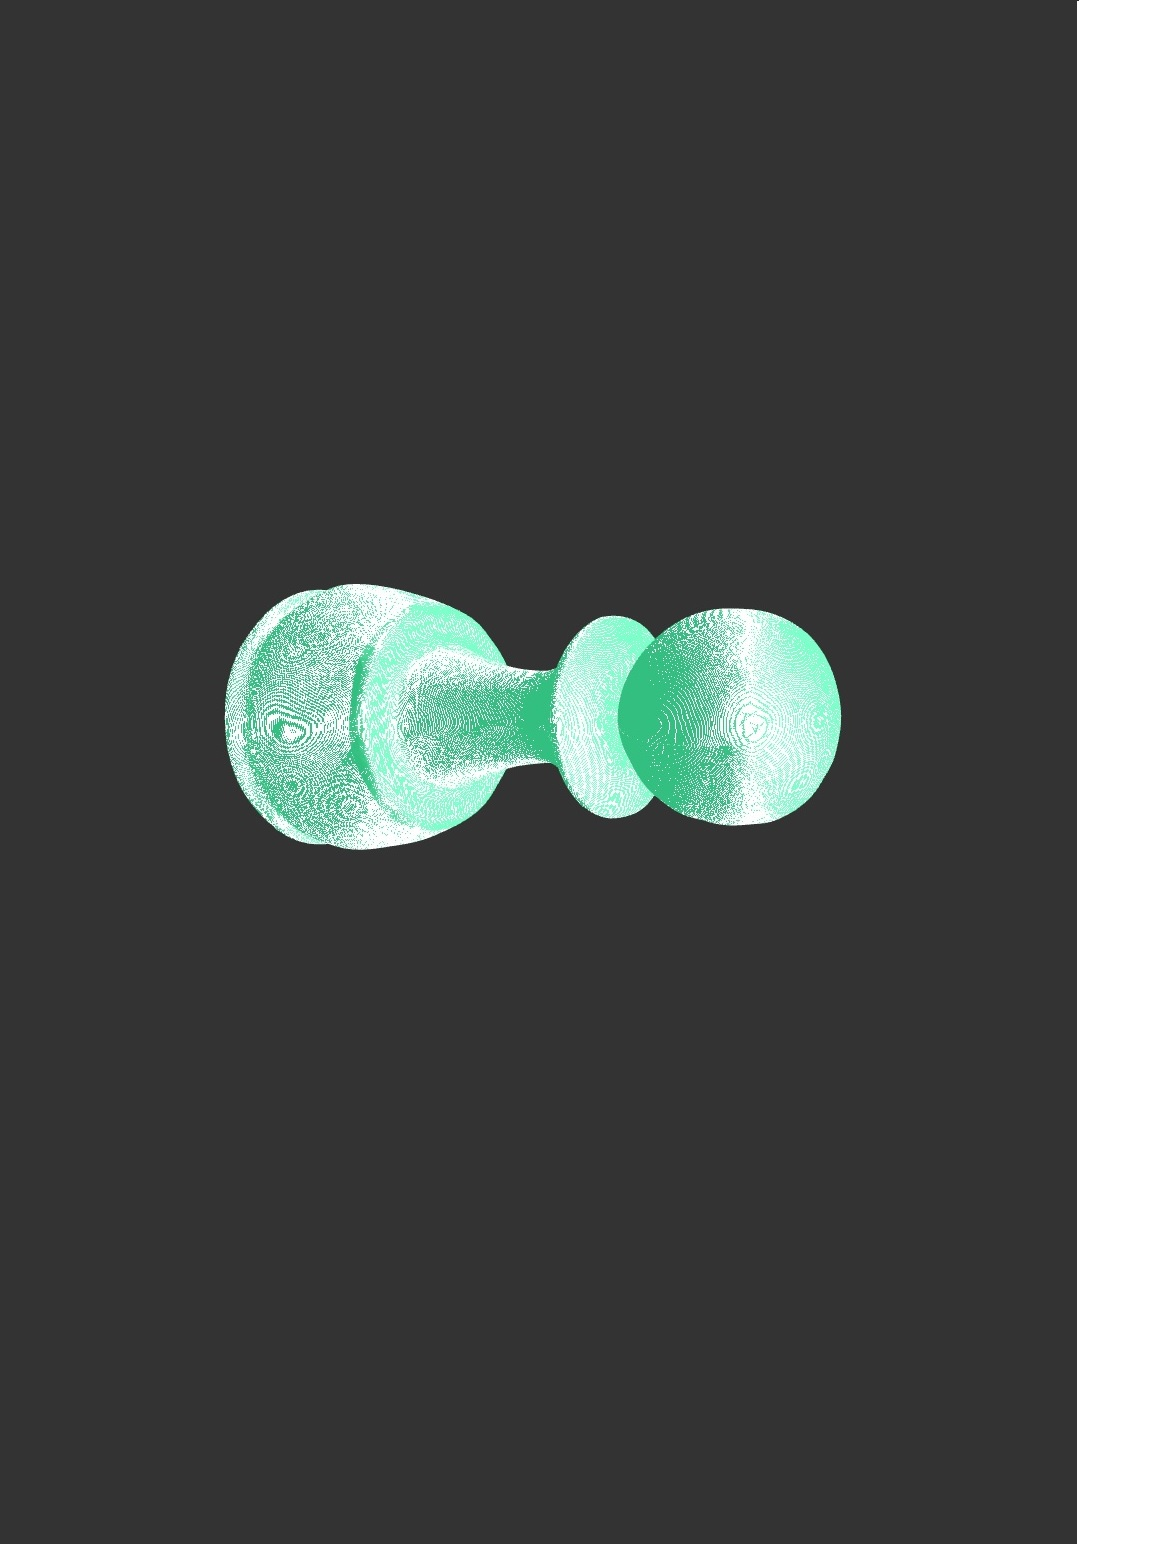
\includegraphics[width=1.0\textwidth]{pBadRenderSideways.jpg}
	\caption{High Resolution image of first attempt at pixel synchronization subsurface scattering approximation.}
	\label{pic:bigBadRender}
\end{figure}


\end{document}